\documentclass[11pt,a4paper]{article}

% ---------- Packages ----------
\usepackage[a4paper,top=2.5cm,bottom=2.5cm,left=2.5cm,right=2.3cm,headheight=14pt]{geometry}
\usepackage[T1]{fontenc}
\usepackage[utf8]{inputenc}
\usepackage{lmodern}
\usepackage{microtype}
\usepackage{graphicx}
\usepackage{xcolor}
\usepackage{colortbl}
\usepackage{booktabs}
\usepackage{tabularx}
\usepackage{longtable}
\usepackage{array}
\usepackage{enumitem}
\usepackage{caption}
\usepackage{subcaption}
\usepackage{float}
\usepackage{fancyhdr}
\usepackage{listings}
\usepackage{tikz}
\usetikzlibrary{positioning,fit,backgrounds,arrows.meta,calc}
\usepackage[numbers,sort&compress]{natbib}
\usepackage[hidelinks]{hyperref}
\usepackage{url}
\usepackage{titlesec}

% ---------- Colours (restrained palette) ----------
\definecolor{accent}{RGB}{31,56,100}
\definecolor{codebg}{RGB}{246,246,246}
\definecolor{codeframe}{RGB}{200,200,200}
\definecolor{codekw}{RGB}{31,56,100}
\definecolor{codecom}{RGB}{90,110,90}
\definecolor{codestr}{RGB}{120,60,40}

% ---------- Layout ----------
\setlength{\parskip}{4pt}
\setlength{\emergencystretch}{3em}
\hbadness=5000
\setlength{\parindent}{0pt}
\renewcommand{\arraystretch}{1.15}
\setlist{itemsep=1pt,topsep=3pt}
\captionsetup{font=small,labelfont=bf,skip=5pt}
\titleformat{\section}{\Large\bfseries\color{accent}}{\thesection}{0.8em}{}
\titleformat{\subsection}{\large\bfseries\color{accent}}{\thesubsection}{0.8em}{}
\titleformat{\subsubsection}{\normalsize\bfseries}{\thesubsubsection}{0.8em}{}
\titlespacing*{\section}{0pt}{16pt}{6pt}
\titlespacing*{\subsection}{0pt}{11pt}{4pt}

\pagestyle{fancy}
\fancyhf{}
\fancyhead[L]{\small MULTYVERS -- Campus Event Management Platform}
\fancyhead[R]{\small CS202C Software Systems Lab, IIT Dharwad}
\fancyfoot[C]{\small\thepage}
\renewcommand{\headrulewidth}{0.4pt}
\fancypagestyle{plain}{\fancyhf{}\fancyfoot[C]{\small\thepage}\renewcommand{\headrulewidth}{0pt}}

% ---------- Listings ----------
\lstdefinestyle{mv}{
  basicstyle=\ttfamily\footnotesize,
  backgroundcolor=\color{codebg},
  frame=single, rulecolor=\color{codeframe},
  keywordstyle=\color{codekw}\bfseries,
  commentstyle=\color{codecom}\itshape,
  stringstyle=\color{codestr},
  numbers=left, numberstyle=\tiny\color{gray}, numbersep=6pt,
  breaklines=true, breakatwhitespace=false,
  columns=fullflexible, keepspaces=true,
  xleftmargin=14pt, framexleftmargin=12pt,
  aboveskip=6pt, belowskip=4pt, showstringspaces=false,
  captionpos=b
}
\lstdefinelanguage{SQLmv}{
  morekeywords={CREATE,TABLE,IF,NOT,EXISTS,PRIMARY,KEY,AUTOINCREMENT,TEXT,INTEGER,NULL,UNIQUE,CHECK,IN,DEFAULT,FOREIGN,REFERENCES,INDEX,ON,TIMESTAMP,COLLATE,NOCASE,PRAGMA,SELECT,FROM,WHERE,AND,INSERT,INTO,VALUES,UPDATE,SET,JOIN},
  sensitive=false, morecomment=[l]{--}, morestring=[b]'
}
\lstset{style=mv}

\urlstyle{tt}
\usepackage{xstring}
\DeclareRobustCommand{\code}[1]{\texttt{\StrSubstitute{\detokenize{#1}}{\string_}{\_\allowbreak}}}
% Visible marker for information the team still has to supply
\newcommand{\placeholder}[1]{\textbf{\textcolor{red!60!black}{[#1]}}}

\begin{document}

% ================= TITLE PAGE =================
\begin{titlepage}
\centering
\vspace*{1.2cm}
{\large Indian Institute of Technology Dharwad}\\[4pt]
{\normalsize Department of Computer Science and Engineering}\\[1.6cm]
{\normalsize CS202C -- Software Systems Lab}\\[0.4cm]
{\normalsize Project Report}\\[1.2cm]
\rule{\textwidth}{0.8pt}\\[0.5cm]
{\fontsize{30}{34}\selectfont\bfseries\color{accent} MULTYVERS}\\[0.3cm]
{\Large Campus Event Management Platform}\\[0.2cm]
{\normalsize A role-based web application built with Python, Flask and SQLite}\\[0.4cm]
\rule{\textwidth}{0.8pt}\\[1.6cm]



\begin{tabular}{@{}l l l@{}}
\textbf{Submitted by:} 
& \placeholder{Kanikala Pranav Tej} 
& \placeholder{MC25BT006}\\

& \placeholder{Gandham Sri Krishna Venkata Sankar} 
& \placeholder{MC25BT025}\\

& \placeholder{Majji Rupesh Babu} 
& \placeholder{MC25BT003}\\

& \placeholder{Chitti Lakshmi Karthik Reddy} 
& \placeholder{MC25BT010}\\

& \placeholder{Bata Teja Srinivas} 
& \placeholder{MC25BT019}\\[6pt]

\textbf{Course instructor:} 
& \multicolumn{2}{l}{\placeholder{Dr. Suman Dutta}}\\[6pt]

\textbf{Repository:} 
& \multicolumn{2}{l}{\url{https://github.com/kanikalapranavtej/MULTYVERS}}\\

\textbf{Date:} & \multicolumn{2}{l}{November 2026}
\end{tabular}

\vfill
\end{titlepage}

\pagenumbering{roman}
\tableofcontents
\clearpage
\listoffigures
\listoftables
\clearpage
\pagenumbering{arabic}

% ================= ABSTRACT =================
\section*{Abstract}
\addcontentsline{toc}{section}{Abstract}
MULTYVERS is a role-based campus event management platform developed to bring the
complete event lifecycle into one connected web application. Instead of handling event
announcements, approvals, venue coordination, registrations, participant lists and attendance
through separate tools, the platform links these activities to a shared database and applies
consistent rules at each stage. The application provides dedicated portals for students,
organizers and administrators. Students can discover approved events, filter listings, view event
details, register or cancel a registration, and mark their attendance by scanning an event QR
code. Organizers can request access, create and update event proposals after approval, check
venue availability, review participant lists, generate attendance QR codes, export records and
inspect event analytics. Administrators supervise the platform by approving organizer accounts
and event proposals, maintaining venues and categories, and managing student accounts.

The system is implemented using Python and Flask. Flask routes and blueprints handle requests
and role checks; Jinja2, HTML, CSS and JavaScript provide the browser interface; and SQLite
stores users, events, venues, registrations and attendance. Validation is performed both in the
application logic and through database constraints—for example, to prevent duplicate
registrations, capacity violations and overlapping venue bookings. This report focuses primarily
on how a user moves through MULTYVERS, how each portal supports its tasks, how the major
features are implemented, and how the data moves between the interface, server and database.
The functional test suite has a recorded result of 222 passing tests. The report also documents
the development workflow and clearly distinguishes completed features from work that remains which has not yet been carried out.

\section{Introduction}

\subsection{Background and problem statement}
On a campus, the work around a single event is usually spread over several channels. An
announcement goes out on a messaging group, registrations are collected through a form,
the venue is booked by email, the approval is a signature or a message, and attendance is
taken on paper. Each step is simple, but nothing connects them. Organizers cannot easily see how many
students have registered, two events can end up in the same hall at the same time, and
attendance cannot be matched against the registration list.

MULTYVERS tries to replace this with a single system in which the state of an event
(pending, approved, cancelled), its venue, its registrations and its attendance are stored
together and checked against each other.

\subsection{Objective}
The objective was to build a centralised, role-based campus event management system in which

\begin{itemize}
  \item \textbf{students} can find approved events, register, cancel, and check in at the event;
  \item \textbf{organizers} can propose events, manage participants, generate a QR code for
        attendance and view analytics for their events;
  \item \textbf{administrators} can approve or reject organizers and events, manage venues, categories
        and student accounts, and see platform-wide numbers.
\end{itemize}

\subsection{Scope}
The implemented system is a server-rendered web application intended to run locally with the Flask
development server. It does not include e-mail or push notifications, online payments, or a production
deployment. These are listed as future scope in Section~\ref{sec:conclusion}.

\subsection{Organisation of this report}
Section~\ref{sec:tech} lists the technologies that are actually used in the repository.
Section~\ref{sec:arch} describes the architecture and database. Section~\ref{sec:impl}
explains the implementation by feature, with code excerpts. Section~\ref{sec:course} connects
the work to the course topics. Section~\ref{sec:testing} covers functional testing,
Section~\ref{sec:results} presents screenshots of the running application, followed by the conclusion and references.

% ================= 2 TECHNOLOGIES =================
\section{Technologies Used}
\label{sec:tech}
Only technologies whose use could be confirmed in the repository are listed.
Table~\ref{tab:tech} gives each one together with its role; the exact Python packages come from
\code{requirements.txt} (Table~\ref{tab:req}).

\begin{table}[H]
\centering
\caption{Technologies used in MULTYVERS and where they appear.}
\label{tab:tech}
\small
\begin{tabularx}{\textwidth}{@{}p{2.9cm}X@{}}
\toprule
\textbf{Technology} & \textbf{Use in the project}\\
\midrule
Python 3~\cite{pythondocs} & All server-side code under \code{app/}; database initialisation script; tests.\\
Flask~\cite{flaskdocs,grinberg2018flask} & Web framework: routing, request/response handling, Jinja2 rendering, sessions.\\
Flask Blueprints & The application is split into 16 blueprints (one per feature area), registered in \code{create_app()}.\\
Flask-Login~\cite{flasklogin} & Session-based login, \code{login_required}, \code{current_user}.\\
Flask-WTF~\cite{flaskwtf} & \code{CSRFProtect} for CSRF tokens on every state-changing request.\\
Werkzeug & Password hashing (\code{generate_password_hash}, \code{check_password_hash}).\\
Jinja2~\cite{jinjadocs} & Server-side templates with a shared \code{base.html} and reusable components.\\
HTML, CSS~\cite{mdn} & Page structure and styling (nine CSS files; dark theme with a light-theme toggle).\\
JavaScript & Client-side behaviour in \code{static/js}: calls to the JSON API with \code{fetch}, filtering, QR scanner page, charts.\\
Chart.js~\cite{chartjs} & Charts on the organizer analytics page (loaded from a CDN in \code{analytics/dashboard.html}).\\
SQLite, SQL~\cite{sqlitedocs} & Single-file relational database; schema in \code{database/schema.sql}; Python \code{sqlite3} module.\\
\code{qrcode}~\cite{pythonqrcode} + Pillow & Generates the attendance QR code as a PNG.\\
\code{itsdangerous}~\cite{itsdangerousdocs} & Signs and time-limits the token that is encoded in the QR code.\\
CSV (\code{csv} module) & Export of participants, attendance and analytics.\\
pytest~\cite{pytestdocs} & 222 functional tests in \code{tests/}.\\
Git~\cite{chacon2014progit}, GitHub & Version control; remote at GitHub with feature branches.\\
Bash scripts & \code{scripts/setup.sh}, \code{run.sh}, \code{test.sh}.\\
venv, VS Code & Virtual environment for dependencies; \code{venv/} and \code{.vscode/} are listed in \code{.gitignore}.\\
\bottomrule
\end{tabularx}
\end{table}

\begin{table}[H]
\centering
\caption{Packages pinned in \code{requirements.txt}.}
\label{tab:req}
\small
\begin{tabularx}{\textwidth}{@{}p{3.9cm}p{2.2cm}X@{}}
\toprule
\textbf{Package} & \textbf{Version} & \textbf{Purpose}\\
\midrule
Flask & 3.1.3 & Web framework\\
Flask-Login & 0.6.3 & User sessions\\
Flask-WTF, WTForms & 1.3.0, 3.3.2 & CSRF protection\\
Werkzeug, Jinja2, MarkupSafe & 3.1.9, 3.1.6, 3.0.4 & Flask dependencies (hashing, templates)\\
itsdangerous, click, blinker & 2.2.0, 8.5.1, 1.9.0 & Flask dependencies (signed tokens, CLI, signals)\\
qrcode, Pillow & 8.2, 13.0.0 & QR image generation\\
pytest (and iniconfig, pluggy, packaging, Pygments, colorama) & 9.2.0 & Test runner and its dependencies\\
\bottomrule
\end{tabularx}
\end{table}

\noindent Flask was chosen because it is small enough to read completely, which suited a lab project in which every
member had to understand the whole request path. SQLite needs no server and ships with Python, so
the project runs after a single \code{pip install}. The trade-off is that SQLite is not designed for many
concurrent writers; we discuss this under future scope.

% ================= 3 ARCHITECTURE =================
\section{System Architecture}
\label{sec:arch}

\subsection{Overview}
MULTYVERS is a server-rendered web application with a thin JSON API behind it. A page is requested
by the browser, Flask finds the matching blueprint route, the route checks the user's role and
runs the business rules against SQLite, and the result comes back either as an HTML page (rendered with
Jinja2) or as JSON that the page's JavaScript displays. Figure~\ref{fig:arch} shows this flow.

\begin{figure}[H]
\centering
\resizebox{\textwidth}{!}{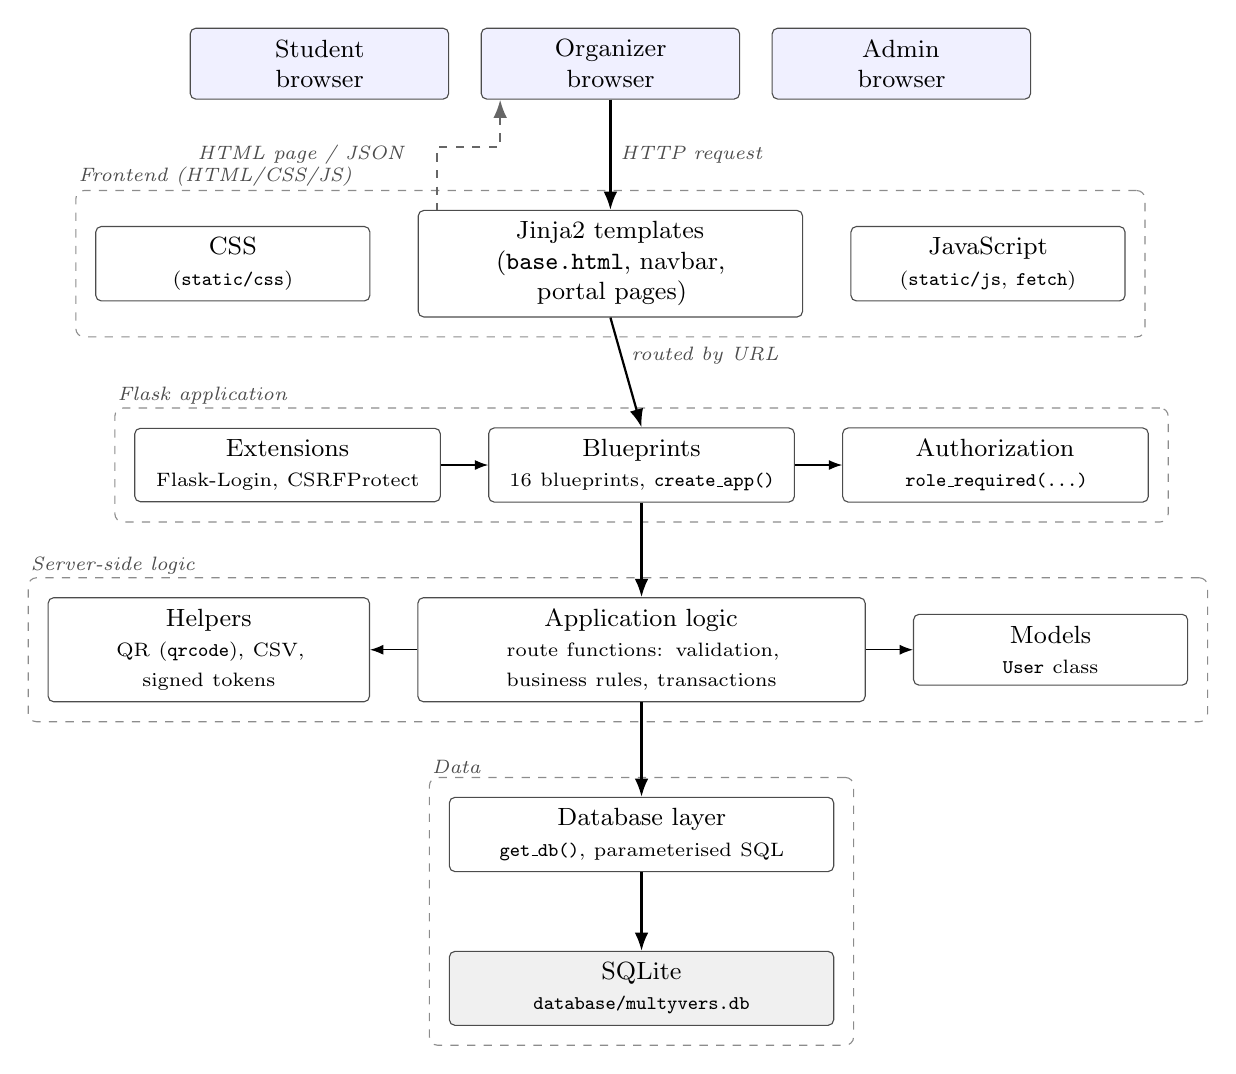
\begin{tikzpicture}[
  font=\small, >=Latex, node distance=6mm,
  box/.style={draw=black!70, rounded corners=2pt, align=center, minimum height=9mm, inner sep=4pt, fill=white},
  layer/.style={draw=black!45, dashed, rounded corners=3pt, inner sep=7pt},
  lab/.style={font=\scriptsize\itshape, text=black!70}
]
% Users
\node[box, fill=blue!6, text width=3.0cm] (stu) {Student\\browser};
\node[box, fill=blue!6, text width=3.0cm, right=4mm of stu] (org) {Organizer\\browser};
\node[box, fill=blue!6, text width=3.0cm, right=4mm of org] (adm) {Admin\\browser};

% Frontend
\node[box, text width=4.6cm, below=14mm of org] (tpl) {Jinja2 templates\\(\texttt{base.html}, navbar, portal pages)};
\node[box, text width=3.2cm, left=6mm of tpl] (css) {CSS\\\scriptsize(\texttt{static/css})};
\node[box, text width=3.2cm, right=6mm of tpl] (js) {JavaScript\\\scriptsize(\texttt{static/js}, \texttt{fetch})};

% Flask
\node[box, text width=3.6cm, below=14mm of tpl, xshift=-4.1cm] (ext) {Extensions\\\scriptsize Flask-Login, CSRFProtect};
\node[box, text width=3.6cm, right=6mm of ext] (bp) {Blueprints\\\scriptsize 16 blueprints, \texttt{create\_app()}};
\node[box, text width=3.6cm, right=6mm of bp] (auth) {Authorization\\\scriptsize\texttt{role\_required(...)}};

% Logic
\node[box, text width=5.4cm, below=12mm of bp] (logic) {Application logic\\\scriptsize route functions: validation, business rules, transactions};
\node[box, text width=3.8cm, left=6mm of logic] (qr) {Helpers\\\scriptsize QR (\texttt{qrcode}), CSV, signed tokens};
\node[box, text width=3.2cm, right=6mm of logic] (mod) {Models\\\scriptsize\texttt{User} class};

% Data
\node[box, text width=4.6cm, below=12mm of logic] (dbl) {Database layer\\\scriptsize\texttt{get\_db()}, parameterised SQL};
\node[box, fill=black!6, text width=4.6cm, below=10mm of dbl] (sql) {SQLite\\\scriptsize\texttt{database/multyvers.db}};

% layers
\begin{scope}[on background layer]
 \node[layer, fit=(tpl)(css)(js), label={[lab, fill=white, anchor=south west, inner sep=1pt]north west:Frontend (HTML/CSS/JS)}] {};
 \node[layer, fit=(ext)(bp)(auth), label={[lab, fill=white, anchor=south west, inner sep=1pt]north west:Flask application}] {};
 \node[layer, fit=(logic)(qr)(mod), label={[lab, fill=white, anchor=south west, inner sep=1pt]north west:Server-side logic}] {};
 \node[layer, fit=(dbl)(sql), label={[lab, fill=white, anchor=south west, inner sep=1pt]north west:Data}] {};
\end{scope}

% request flow
\draw[->, thick] (org.south) -- node[right, lab]{HTTP request} (tpl.north);
\draw[->, thick] (tpl.south) -- node[right, lab, pos=.35]{routed by URL} (bp.north);
\draw[->, thick] (bp.south) -- (logic.north);
\draw[->, thick] (logic.south) -- (dbl.north);
\draw[->, thick] (dbl.south) -- (sql.north);
\draw[->] (ext) -- (bp);
\draw[->] (bp) -- (auth);
\draw[->] (logic) -- (qr);
\draw[->] (logic) -- (mod);
% response flow
\draw[<-, dashed, thick, black!60] ([xshift=-14mm]org.south) -- ++(0,-6mm) -| ([xshift=-2.2cm]tpl.north) ;
\node[lab, anchor=east] at ([xshift=-2.5cm, yshift=7mm]tpl.north) {HTML page / JSON};
\end{tikzpicture}
}
\caption{Architecture of MULTYVERS. Solid arrows are the request path; the dashed arrow is the response returning to the browser as an HTML page or JSON.}
\label{fig:arch}
\end{figure}

\subsection{Application factory and blueprints}
The application is created by \code{create_app()} in \code{app/__init__.py}. It loads
\code{Config}, initialises the extensions and the database helpers, and registers the blueprints.
The blueprints fall into three groups (Table~\ref{tab:bp}): those that return pages, those that
form the JSON API under \code{/api}, and the authentication blueprint under \code{/auth}.

\begin{table}[H]
\centering
\caption{Blueprints registered in \code{create_app()}.}
\label{tab:bp}
\footnotesize
\begin{tabularx}{\textwidth}{@{}p{3.6cm}p{3.0cm}X@{}}
\toprule
\textbf{Blueprint (file)} & \textbf{URL prefix} & \textbf{Responsibility}\\
\midrule
\code{main} (main.py) & \code{/} & Redirects to the portal; \code{/health}; role dashboards (\code{/student|organizer|admin/dashboard})\\
\code{auth} (auth.py) & \code{/auth} & Register, login, organizer request, logout\\
\code{portal_pages} & \code{/} & Portal pages, event create/edit forms, admin event review page\\
\code{pages} & \code{/events} & Public event listing and event detail pages\\
\code{events} & \code{/api/events} & Event CRUD, search, cancel, approve, reject\\
\code{registrations} & \code{/api/registrations} & Register, list own, cancel registration\\
\code{participants} & \code{/api/events} & Participant page, list, CSV export\\
\code{attendance} & \code{/api} & QR generation, attendance marking, report, CSV export\\
\code{attendance_pages} & \code{/} & Organizer attendance page, student scanner page\\
\code{venues}, \code{venue_pages} & \code{/api/venues}, \code{/admin/venues} & Venue CRUD, availability check, admin page\\
\code{category_pages} & \code{/admin/categories} & Category management page\\
\code{organizer_management} & \code{/admin/organizers} & Create, edit, approve, reject, (de)activate, delete organizers\\
\code{admin_students} & \code{/admin/students} & List students, deactivate/reactivate\\
\code{analytics}, \code{analytics_pages} & \code{/api/analytics}, \code{/analytics/dashboard} & Metrics, per-event analytics, CSV export, dashboard page\\
\bottomrule
\end{tabularx}
\end{table}

\begin{lstlisting}[language=Python,caption={Blueprint registration in \texttt{app/\_\_init\_\_.py} (excerpt).},label={lst:init}]
def create_app(config_class=Config):
    app = Flask(__name__)
    app.config.from_object(config_class)

    init_extensions(app)
    init_database(app)

    from app.routes.main import main_bp
    from app.routes.auth import auth_bp
    ...
    app.register_blueprint(main_bp)
    app.register_blueprint(auth_bp)
    app.register_blueprint(events_bp)
    ...
    @app.errorhandler(404)
    def not_found(error):
        return jsonify({"error": "Resource not found"}), 404
    return app
\end{lstlisting}

Passing the configuration class as an argument is what makes the tests possible: each test builds
the application with a \code{DATABASE} path that points at a temporary file (Section~\ref{sec:testing}).

\subsection{Project layout}
\begin{lstlisting}[basicstyle=\ttfamily\footnotesize,numbers=none,caption={Repository layout (generated files omitted).},label={lst:tree}]
MULTYVERS/
  run.py                  # entry point: create_app(), app.run on 127.0.0.1
  requirements.txt
  app/
    __init__.py           # application factory
    config.py  extensions.py  database.py  decorators.py  models.py
    routes/               # 16 blueprints (auth, events, registrations, ...)
    templates/            # base.html, components/, student/, organizer/, admin/, ...
    static/css  static/js
  database/schema.sql  init_db.py  multyvers.db
  tests/                  # 21 test modules + conftest.py + tests_report.docx
  scripts/                # setup.sh  run.sh  test.sh
  docs/  report/  profiling/   # directories present in the repository; profiling/ is empty
\end{lstlisting}

\subsection{Database design}
The database has six tables (\code{users}, \code{categories}, \code{venues}, \code{events},
\code{registrations}, \code{attendance}) and was written as plain SQL in \code{database/schema.sql}.
Figure~\ref{fig:er} shows the tables and their relationships exactly as defined there; no other
tables exist.

\begin{figure}[!htbp]
\centering
\resizebox{\textwidth}{!}{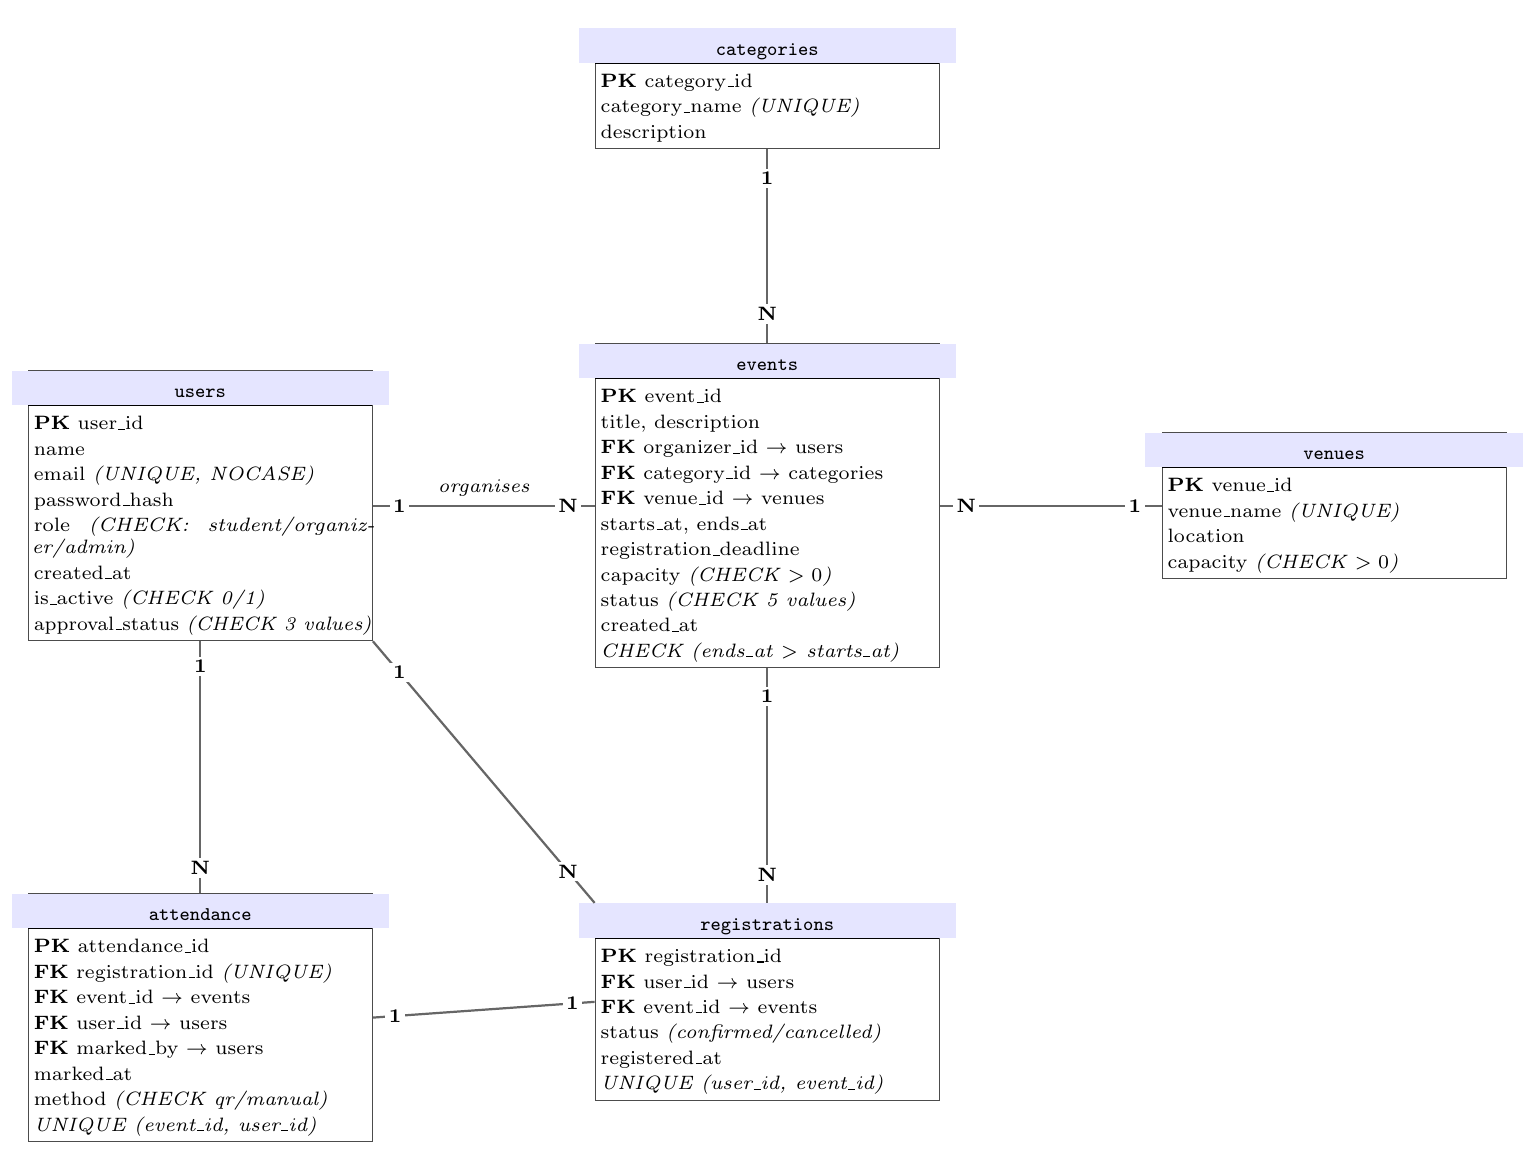
\begin{tikzpicture}[font=\scriptsize, >=Latex,
 ent/.style={draw=black!70, fill=white, inner sep=0pt},
 rel/.style={draw=black!60, thick},
 card/.style={font=\scriptsize\bfseries, fill=white, inner sep=1.2pt}]
\newcommand{\entity}[4]{\node[ent] (#1) at (#2) {\begin{tabular}{@{\hspace{2pt}}p{4.3cm}@{}}
  \multicolumn{1}{@{}c@{}}{\cellcolor{blue!10}\rule{0pt}{3.4mm}\textbf{\texttt{#3}}}\\\hline
  \rule{0pt}{3mm}#4\\[1pt]\end{tabular}};}
\entity{users}{0,0}{users}{\textbf{PK} user\_id\\ name\\ email \textit{(UNIQUE, NOCASE)}\\ password\_hash\\ role \textit{(CHECK: student/organizer/admin)}\\ created\_at\\ is\_active \textit{(CHECK 0/1)}\\ approval\_status \textit{(CHECK 3 values)}}
\entity{events}{7.2,0}{events}{\textbf{PK} event\_id\\ title, description\\ \textbf{FK} organizer\_id $\rightarrow$ users\\ \textbf{FK} category\_id $\rightarrow$ categories\\ \textbf{FK} venue\_id $\rightarrow$ venues\\ starts\_at, ends\_at\\ registration\_deadline\\ capacity \textit{(CHECK $>0$)}\\ status \textit{(CHECK 5 values)}\\ created\_at\\ \textit{CHECK (ends\_at $>$ starts\_at)}}
\entity{categories}{7.2,5.3}{categories}{\textbf{PK} category\_id\\ category\_name \textit{(UNIQUE)}\\ description}
\entity{venues}{14.4,0}{venues}{\textbf{PK} venue\_id\\ venue\_name \textit{(UNIQUE)}\\ location\\ capacity \textit{(CHECK $>0$)}}
\entity{regs}{7.2,-6.3}{registrations}{\textbf{PK} registration\_id\\ \textbf{FK} user\_id $\rightarrow$ users\\ \textbf{FK} event\_id $\rightarrow$ events\\ status \textit{(confirmed/cancelled)}\\ registered\_at\\ \textit{UNIQUE (user\_id, event\_id)}}
\entity{att}{0,-6.5}{attendance}{\textbf{PK} attendance\_id\\ \textbf{FK} registration\_id \textit{(UNIQUE)}\\ \textbf{FK} event\_id $\rightarrow$ events\\ \textbf{FK} user\_id $\rightarrow$ users\\ \textbf{FK} marked\_by $\rightarrow$ users\\ marked\_at\\ method \textit{(CHECK qr/manual)}\\ \textit{UNIQUE (event\_id, user\_id)}}
\draw[rel] (users.east) -- (events.west);
\node[card] at ($(users.east)!0.12!(events.west)$) {1};
\node[card] at ($(users.east)!0.88!(events.west)$) {N};
\node[font=\scriptsize\itshape,above] at ($(users.east)!0.5!(events.west)$) {organises};
\draw[rel] (categories.south) -- (events.north);
\node[card] at ($(categories.south)!0.15!(events.north)$) {1};
\node[card] at ($(categories.south)!0.85!(events.north)$) {N};
\draw[rel] (venues.west) -- (events.east);
\node[card] at ($(venues.west)!0.12!(events.east)$) {1};
\node[card] at ($(venues.west)!0.88!(events.east)$) {N};
\draw[rel] (events.south) -- (regs.north);
\node[card] at ($(events.south)!0.12!(regs.north)$) {1};
\node[card] at ($(events.south)!0.88!(regs.north)$) {N};
\draw[rel] (users.south east) -- (regs.north west);
\node[card] at ($(users.south east)!0.12!(regs.north west)$) {1};
\node[card] at ($(users.south east)!0.88!(regs.north west)$) {N};
\draw[rel] (att.east) -- (regs.west);
\node[card] at ($(att.east)!0.1!(regs.west)$) {1};
\node[card] at ($(att.east)!0.9!(regs.west)$) {1};
\draw[rel] (users.south) -- (att.north);
\node[card] at ($(users.south)!0.1!(att.north)$) {1};
\node[card] at ($(users.south)!0.9!(att.north)$) {N};
\end{tikzpicture}
}
\caption{Entity--relationship diagram derived from \code{database/schema.sql}. \textbf{PK} = primary key, \textbf{FK} = foreign key. Italic text shows constraints. \code{attendance.event_id} and \code{attendance.marked_by} refers \code{events} and \code{users} as listed in the table but are not drawn, to avoid crossing lines.}
\label{fig:er}
\end{figure}

\begin{description}[leftmargin=0pt,labelindent=0pt,style=unboxed]
\item[users:] One table for all three roles; the \code{role} column is restricted by a
\code{CHECK} constraint to \code{student}, \code{organizer} or \code{admin}. Email is
\code{UNIQUE} and case-insensitive (\code{COLLATE NOCASE}). \code{is_active} (0/1) switches an account on or off, and
\code{approval_status} (\code{pending}, \code{approved}, \code{rejected}) is used for the organizer approval process.
\item[events:] Each event refers its organizer (\code{users}), \code{categories} and \code{venues}.
\code{capacity > 0}, \code{ends_at > starts_at} and the five allowed statuses
(\code{draft, pending, approved, rejected, cancelled}) are enforced by \code{CHECK}s. New events default to \code{pending}.
\item[registrations:] Links a student to an event. \code{UNIQUE(user_id, event_id)} makes a duplicate
registration impossible at database level; \code{status} is \code{confirmed} or \code{cancelled}, so cancelling keeps the row.

\item[attendance:] One row per student per event, with both \code{UNIQUE(registration_id)} and
\code{UNIQUE(event_id, user_id)}. \code{method} records how it was marked (\code{qr} or \code{manual}) and \code{marked_by} points to a user.
\item[Indexes:] \code{idx_events_status}, \code{idx_events_category}, \code{idx_registrations_event}, \code{idx_registrations_user}, \code{idx_attendance_event}, \code{idx_attendance_user} and \code{idx_attendance_marked_at}.
\end{description}

\begin{lstlisting}[language=SQLmv,caption={The \code{registrations} table in \code{database/schema.sql}.},label={lst:regsql}]
CREATE TABLE IF NOT EXISTS registrations (
    registration_id INTEGER PRIMARY KEY AUTOINCREMENT,
    user_id INTEGER NOT NULL,
    event_id INTEGER NOT NULL,
    status TEXT NOT NULL DEFAULT 'confirmed'
        CHECK(status IN ('confirmed', 'cancelled')),
    registered_at TIMESTAMP DEFAULT CURRENT_TIMESTAMP,
    FOREIGN KEY(user_id) REFERENCES users(user_id),
    FOREIGN KEY(event_id) REFERENCES events(event_id),
    UNIQUE(user_id, event_id)
);
\end{lstlisting}

SQLite does not enforce foreign keys unless asked, so \code{get_db()} runs \code{PRAGMA foreign_keys = ON}
on every new connection (Listing~\ref{lst:getdb}).

\subsection{Request lifecycle: one example}
When a student presses \emph{Register for event}, the page's JavaScript sends
\code{POST /api/registrations/} with the event id and the CSRF token. Flask-WTF checks the token,
\code{role_required("student")} checks the session, and the view validates the event and writes
to the \code{registrations} table inside a transaction. The JSON answer
(\code{201 Successfully registered} or an error such as \code{409 already registered}) is shown on the
page, which then updates the button to \emph{Cancel registration}.

% ================= 4 IMPLEMENTATION =================
\section{Implementation Details}
\label{sec:impl}

\subsection{Application initialisation}
\code{run.py} builds the application with \code{create_app()} and starts the development server on
\code{127.0.0.1}; debug mode is off unless \code{MULTYVERS_DEBUG=true}. \code{Config} (in
\code{config.py}) reads the secret key from \code{MULTYVERS_SECRET_KEY}, sets the database path, and
turns on \code{HttpOnly} and \code{SameSite=Lax} cookies and CSRF protection. \code{init_app()} in
\code{database.py} registers the connection teardown, runs a small migration that adds the
\code{is_active} and \code{approval_status} columns to databases created before they existed, and makes sure
the single administrator account exists.

\begin{lstlisting}[language=Python,caption={Per-request database connection (\code{app/database.py}).},label={lst:getdb}]
def get_db():
    """Get a database connection for the current request."""
    if "db" not in g:
        connection = sqlite3.connect(current_app.config["DATABASE"], timeout=10)
        connection.row_factory = sqlite3.Row
        connection.execute("PRAGMA foreign_keys = ON")
        connection.execute("PRAGMA busy_timeout = 10000")
        g.db = connection
    return g.db
\end{lstlisting}

The connection is stored in Flask's request-scoped object \code{g}, so every query in one request shares
one connection, and \code{close_db()} closes it when the request context ends.
All SQL in the project uses \code{?} placeholders, never string formatting of user input.


\subsection{Authentication and authorization}
\textbf{Registration and login:} Students register themselves; the form checks that all
fields are present, that the two passwords match, that the password has at least eight characters
and that the email is not taken, and then stores a Werkzeug password hash. Outside test mode,
student and organizer addresses must end in \code{@multyvers.in}, and \code{admin@multyvers.in} is reserved.
At login the password hash is checked and the user is logged in with Flask-Login; if the
\code{next} parameter is present it is only followed when it points to the same host.

\textbf{Roles:} The \code{User} class in \code{models.py} wraps a database row. Its \code{is_active}
property is true only if the account flag is set \emph{and}, for organizers, the approval status is
\code{approved}. This one rule makes deactivated accounts and pending or rejected organizers unable to
log in (the login view shows a different message for each case).

\begin{lstlisting}[language=Python,caption={\code{app/models.py}: an organizer is active only after approval.},label={lst:isactive}]
@property
def is_active(self):
    return self._account_active and (
        self.role != "organizer" or self.approval_status == "approved"
    )
\end{lstlisting}

\textbf{Authorization:} uses one decorator, \code{role_required}, applied to every protected view
(Listing~\ref{lst:role}). It stacks \code{login_required} (unauthenticated users go to the login page), then returns
HTTP 403 if the account is inactive or the role is not in the allowed list. Admin-only views, such as venue
CRUD and event approval, are therefore unreachable for students and organizers even if the URL is typed manually.
Ownership checks are added where needed: for example an organizer can only update, cancel or view
participants of \emph{their own} events.

\begin{lstlisting}[language=Python,caption={\code{app/decorators.py}.},label={lst:role}]
def role_required(*roles):
    def decorator(view_function):
        @wraps(view_function)
        @login_required
        def decorated_function(*args, **kwargs):
            if not current_user.is_active:
                abort(403)
            if current_user.role not in roles:
                abort(403)
            return view_function(*args, **kwargs)
        return decorated_function
    return decorator
\end{lstlisting}

\subsection{Student functionality}
After login a student lands on the dashboard (\code{/student/portal}), which shows the number of active
registrations and a table of their events with a \emph{Cancel registration} action. The event listing
(\code{/events}, \code{pages.py}) shows only events with status \code{approved}, with a text search, a category
filter, sorting (upcoming, latest, popular), an optional date range and pagination; the same filters are
available on the JSON endpoint \code{GET /api/events}. The detail page shows date, venue, organizer, registered
count and the registration deadline, and its button switches between \emph{Register for event} and \emph{Cancel registration}.
The \emph{QR} entry in the student menu opens the scanner page used for attendance (Section~\ref{sec:attimpl}).
Student actions are limited to students by \code{role_required("student")}.

\subsection{Organizer functionality}
Organizers cannot register directly. They submit an \emph{organizer request}
(\code{/auth/organizer-request}), which creates a user with \code{approval_status = pending}; the request becomes
usable only after an administrator approves it. An approved organizer works from four pages:

\begin{itemize}
  \item the dashboard with counts of own, approved and pending events and a table with edit and cancel actions;
  \item the event form for creating or editing an event with category, venue, capacity and three date-times;
  \item the participants page (event selector, status filter, search, pagination, CSV export);
  \item the attendance page (QR generation and attendance report) and the analytics dashboard.
\end{itemize}

\subsection{Admin functionality}
The administrator is a single account, \code{admin@multyvers.in}, created at start-up by
\code{ensure_default_admin()} from the \code{MULTYVERS_ADMIN_PASSWORD} environment variable (default
\code{password} if it is unset); any other row with the admin role is removed, and login refuses other admin
addresses outside test mode. The admin portal offers an overview with platform counts, and five
management pages:

\begin{itemize}
  \item \textbf{Organizers:} create accounts directly, edit name/email, approve or reject requests,
        deactivate or delete (\code{organizer_management.py}).
  \item \textbf{Events:} review the pending events with \emph{Approve} and \emph{Reject}
        (a \code{PATCH} request to the events API).
  \item \textbf{Venues} and \textbf{Categories:} create, edit, delete; venues also have an availability checker.
  \item \textbf{Students:} search and deactivate/reactivate accounts (\code{admin_students.py}).
\end{itemize}

\subsection{Event management}
Event creation is \code{POST /api/events/} (organizer only). The view validates the JSON body step by step:
required fields; title; numeric fields (\code{parse_positive_integer} rejects booleans, floats and
non-positive values); ISO~8601 dates with consistent timezone information; end after start; registration
deadline not after the start and still in the future; the category and venue exist; event capacity does not
exceed venue capacity; and no overlapping booking of the venue. Only then is the event inserted with status
\code{pending}. The venue check is shared by create, update and approval:

\begin{lstlisting}[language=Python,caption={Venue overlap check (\code{app/routes/events.py}, abridged).},label={lst:conflict}]
def check_venue_conflict(db, venue_id, starts_at, ends_at, exclude_event_id=None):
    query = """SELECT event_id, title, starts_at, ends_at FROM events
               WHERE venue_id = ? AND status IN ('pending', 'approved')"""
    ...
    for event in events:
        existing_start = datetime.fromisoformat(event["starts_at"]).astimezone()
        existing_end = datetime.fromisoformat(event["ends_at"]).astimezone()
        if requested_start < existing_end and requested_end > existing_start:
            return event
    return None
\end{lstlisting}

Two bookings overlap exactly when each starts before the other ends, which is the condition in the last
\code{if}. Cancelled and rejected events do not block a venue. An organizer may update or cancel an event only
while it is \code{pending}; once an admin has decided, the event is fixed. Approval is performed by
\code{review_event()}, which re-runs the venue check (another event may have been approved for the same slot in the
meantime) and then updates the row with \code{WHERE status = 'pending'}, so an event cannot be reviewed twice.

\subsection{Registration management}
Registration is the most constraint-heavy operation (\code{registrations.py}, Listing~\ref{lst:reg}). The view opens
a write transaction with \code{BEGIN IMMEDIATE}, loads the event, and then applies the rules in order:
the event must exist and be \code{approved}; the deadline must not have passed; the student must not
already hold a confirmed registration (HTTP 409); and the number of confirmed registrations must be lower than
the capacity (HTTP 409). A previously cancelled registration is re-activated instead of inserting a second row, because of
the \code{UNIQUE(user_id, event_id)} constraint. Cancellation (\code{DELETE /api/registrations/<event_id>}) sets
the status to \code{cancelled}.

\begin{lstlisting}[language=Python,caption={\code{register_for_event()} in \code{app/routes/registrations.py} (abridged).},label={lst:reg}]
db.execute("BEGIN IMMEDIATE")   # prevent capacity race conditions
event = db.execute("SELECT event_id, registration_deadline, capacity, status "
                   "FROM events WHERE event_id = ?", (event_id,)).fetchone()
if event is None or event["status"] != "approved":
    db.rollback(); return jsonify({"error": "Event not found."}), 404
...
if existing and existing["status"] == "confirmed":
    db.rollback()
    return jsonify({"error": "You are already registered for this event."}), 409
registered_count = db.execute("SELECT COUNT(*) AS total FROM registrations "
        "WHERE event_id = ? AND status = 'confirmed'", (event_id,)).fetchone()["total"]
if registered_count >= event["capacity"]:
    db.rollback()
    return jsonify({"error": "Event registration capacity is full."}), 409
\end{lstlisting}

\subsection{Attendance management and QR code functionality}
\label{sec:attimpl}
Attendance uses a QR code shown by the organizer and scanned by each student:

\begin{enumerate}
  \item The organizer selects an approved event on the attendance page and presses \emph{Generate QR Code}.
        \code{GET /api/events/<id>/attendance/qr} checks that the organizer owns the event (admins may
        access any) and that it is approved, creates a signed token with
        \code{URLSafeTimedSerializer} (secret key plus a fixed salt, payload \code{\{event_id, purpose\}}), encodes the
        token with the \code{qrcode} library and returns a PNG.
  \item A student opens the scanner page, which uses the device camera and sends the decoded text to
        \code{POST /api/attendance/mark}.
  \item The server verifies the signature and age (24~hours), checks that the event is approved, that the
        current time lies between the event's start and end, that the student has a \emph{confirmed}
        registration, and that attendance has not already been recorded. Only then is a row inserted into
        \code{attendance} with method \code{qr}.
\end{enumerate}

\begin{lstlisting}[language=Python,caption={Token creation and QR image generation (\code{app/routes/attendance.py}).},label={lst:qr}]
token = get_token_serializer().dumps({"event_id": event_id,
                                      "purpose": "attendance"})
qr_image = qrcode.make(token)
image_buffer = BytesIO()
qr_image.save(image_buffer, format="PNG")
image_buffer.seek(0)
return send_file(image_buffer, mimetype="image/png",
                 download_name=f"event_{event_id}_attendance_qr.png")
\end{lstlisting}

Because the token is signed, a student cannot produce a valid QR for another event, and because marking
happens only inside the event time window with a confirmed registration, the code is useless to someone who
did not register or is not present during the event. The marking view also opens its transaction with
\code{BEGIN IMMEDIATE}, and the two \code{UNIQUE} constraints on \code{attendance} act as a second barrier against double
entries; an \code{IntegrityError} is turned into a clean 409 response. The organizer's attendance table lists
name, email, time and method and can be exported as CSV. The schema also allows the method \code{manual}; the
routes we reviewed record attendance only through the QR path.

\subsection{Participant management}
\code{GET /api/events/<id>/participants} returns the registrations of an event together with the attendance
status of each participant (\emph{Present}, \emph{Pending}, or absent after the event ends), supports a status
filter, search over name and email, and pagination, and is used by the participants page.
\code{.../participants/export} returns the same data as CSV.

\subsection{Venue management}
Admins create, edit and delete venues (\code{venues.py}). A venue cannot be deleted while any event refers to it
(HTTP 409). \code{GET /api/venues/availability} is available to admins and organizers: it takes a venue and a
time range and returns whether the slot is free, using the same overlap rule as Listing~\ref{lst:conflict};
the organizer's event form calls it from the \emph{Check Availability} button.

\subsection{Analytics and CSV exports}
\code{analytics.py} provides \code{/api/analytics/overview} (totals of events by status, registrations, attendance
and attendance rate, per-event and per-category figures), \code{/events/<id>} for one event and
\code{/export} for CSV. Organizers see only their own events; admins see all. \code{analytics.js} draws the charts with
Chart.js. All three CSV exports pass every cell through \code{safe_csv_value()}, which prefixes cells starting with
\code{=}, \code{+}, \code{-} or \code{@} with an apostrophe, so that a malicious name such as \code{=cmd()} is not executed as a formula
when the file is opened in a spreadsheet.

\begin{lstlisting}[language=Python,caption={CSV formula-injection guard (repeated in \code{analytics.py}, \code{attendance.py} and \code{participants.py}).},label={lst:csv}]
def safe_csv_value(value):
    """Prevent spreadsheet formula injection."""
    value = "" if value is None else str(value)
    if value.startswith(("=", "+", "-", "@", "\t", "\r")):
        return "'" + value
    return value
\end{lstlisting}

\subsection{Database interaction}
Database access is written as direct SQL in the view functions through \code{sqlite3} and the
\code{get_db()} helper; there is no ORM. Reads use \code{sqlite3.Row} so columns can be accessed by name. Writes follow the
same pattern throughout: \code{try}, execute, \code{commit}; \code{except sqlite3.IntegrityError} rolls back and
returns a 400/409 message; any other exception rolls back and is re-raised so that the 500 handler logs it.
Combining the \code{CHECK}/\code{UNIQUE}/foreign-key constraints in the schema with the checks in the views means that
rules like ``no duplicate registration'' hold even if one of the two layers were bypassed.

% ================= 5 COURSE CONCEPTS =================

\section{Complete User Workflow}
\label{sec:user-flow}
This section explains the intended use of MULTYVERS from the first login to the completion
of an event. The three portals are connected: an action taken by one role changes the information
shown to the other roles because all of them use the same SQLite database. The workflow is
therefore not three separate applications; it is one event process with different permissions.

\subsection{Step 1: Entering the platform and accessing the correct portal}
A user opens the application in a browser and reaches the login page. A student can create an
account through student registration and then sign in. An organizer first submits an organizer
request; this account remains pending until an administrator reviews it. The administrator signs
in through the admin account created during application initialisation. After successful login,
the application uses the authenticated user's role to direct the user to the appropriate dashboard.
The navigation menu is also adapted to that role, so each user sees the pages relevant to their
responsibilities.

\subsection{Step 2: Organizer account approval}
An organizer who is new to the platform submits the organizer request form with the required
details. The request is stored with a pending approval status. The administrator opens Organizer
Management, reviews the request and chooses Approve or Reject. Approval changes the
organizer's account state and permits access to organizer features; a pending or rejected organizer
cannot use the protected organizer portal. This approval step is performed before the organizer
can publish event proposals.

\subsection{Step 3: Creating and submitting an event}
After approval, the organizer opens the event creation form. The organizer enters the event title
and description, chooses a category and venue, and supplies the start time, end time, registration
deadline and participant capacity. Before submission, the venue availability checker can be used
to inspect the selected time slot. When the organizer submits the form, the server validates the
required fields, date order, deadline, category, venue and capacity. It also checks whether another
pending or approved event already occupies the same venue during an overlapping interval.
If the details pass validation, the event is saved with pending status; it is not immediately shown
as an approved event to students.

\subsection{Step 4: Administrative review of the event}
The administrator opens Event Review to see proposals awaiting a decision. The administrator
can inspect the submitted event and approve or reject it. The venue conflict check is repeated at
approval time because another event may have been added after the original proposal was
submitted. An approved event becomes available in the student event listing. A rejected event
does not appear as an approved event for student registration. This two-stage process—organizer
submission followed by administrator review—keeps event publication under administrative
control.

\subsection{Step 5: Student discovery and registration}
A student signs in and opens the Events page. The listing displays approved events and provides
search, category filtering, sorting and date-range filtering to help locate a suitable event. Selecting
an event opens its detail page, where the student can inspect the description, organizer, venue,
schedule, registration deadline and available capacity. The student selects Register for event.
The server checks that the event is approved, the deadline is still open, the student does not
already have a confirmed registration and the event has not reached its capacity. If the checks
pass, a registration record is saved and the interface reflects the confirmed registration. The
student can later cancel the registration; cancellation changes its status rather than creating a
second registration record.

\subsection{Step 6: Organizer checks the participant list}
The organizer opens the Participants page and selects one of their own events. The page displays
the registered participants and their attendance state. The organizer can search by participant
name or e-mail address, filter the list by status, move through paginated results and export the
participant information as a CSV file. This page uses the same registration records created by
students, so the organizer does not need to collect a separate registration form or manually
reconcile another list.

\subsection{Step 7: Recording attendance using the QR code}
During the event, the organizer opens the Attendance page, selects the approved event and
generates its QR code. The application creates a signed, time-limited token for that event and
returns it as a QR image. A student who has a confirmed registration opens the attendance
scanner page and scans the organizer-displayed code using the device camera. The decoded token
is sent to the server, where its signature and age are checked. The server also verifies that the
event is approved, the current time is within the event's start and end window, the student has a
confirmed registration and attendance has not already been recorded. Only after these checks
does the system create an attendance record. The QR code is therefore generated by the
organizer and scanned by the student; it is not a personal QR ticket issued to each student.

\subsection{Step 8: Reviewing attendance and analytics}
After check-in, the organizer can return to the Attendance and Participants pages to review who
is present and when attendance was marked. The organizer can export attendance information
as CSV. The Analytics dashboard presents event and category summaries, registration totals,
attendance totals and attendance rates using summary cards and charts. Organizers see analytics
for their own events, while administrators can inspect platform-wide figures. These views
reuse the event, registration and attendance data already stored by the application.

\subsection{Step 9: Ongoing platform administration}
The administrator maintains the supporting data required by the event workflow. Venue
Management allows venues to be created, edited and removed, and includes an availability
check. A venue that is referenced by an event cannot be deleted. Category Management keeps
the categories available in event forms. Student Management provides account search and
deactivation or reactivation controls. The admin dashboard gives a consolidated view of
platform activity, including users, organizers, pending requests and events.

\subsection{Workflow summary}
The complete lifecycle can be read as the following sequence:
\begin{enumerate}[leftmargin=*,label=\textbf{\arabic*.}]
  \item Student and organizer accounts are created; organizer access waits for admin approval.
  \item The approved organizer creates an event proposal and selects a venue and schedule.
  \item The application validates the proposal and stores it as pending.
  \item The administrator reviews the proposal and approves or rejects it.
  \item Students discover approved events and register before the deadline and capacity are reached.
  \item Organizers review the resulting participant list and prepare attendance.
  \item The organizer displays a generated QR code; registered students scan it during the event.
  \item The application records attendance, and organizers review reports and analytics.
  \item Administrators continue maintaining organizers, venues, categories and student accounts.
\end{enumerate}
At each stage, the browser sends a request to Flask, the relevant route checks the user's role
and validates the requested operation, and SQLite stores or retrieves the records. The resulting
HTML page or JSON response is then shown in the browser. This shared request-and-data flow
is what connects the three portals into one event management process.

\section{Use of Relevant Course Concepts}
\label{sec:course}
The project applies the course concepts that directly supported implementation and delivery.
Python was used for server-side logic, database operations and tests. HTML, CSS and JavaScript
were used to build the browser interface and its interactive features. Unix command-line tools
and Bash scripts supported setup, execution and testing. Git was used to maintain the shared
codebase and integrate feature branches. \LaTeX{} was used to prepare this report.

\begin{table}[H]
\centering
\caption{Relevant course concepts applied in MULTYVERS.}
\label{tab:course}
\small
\begin{tabularx}{\textwidth}{@{}p{3.0cm}p{2.0cm}X@{}}
\toprule
\textbf{Concept} & \textbf{Application} & \textbf{Where it appears}\\
\midrule
Python programming & Core implementation & Flask routes, validation helpers, database access and pytest tests.\\
HTML, CSS and JavaScript & User interface & Role-specific Jinja2 pages, shared navigation, styling, filtering, QR scanner and analytics charts.\\
Unix and Bash & Project workflow & Virtual-environment setup, dependency installation, application startup and test execution.\\
Git and version control & Team development & Feature branches, commits and merges used to develop and integrate major modules.\\
\LaTeX{} & Documentation & Structured report with figures, tables, code excerpts and references.\\
\bottomrule
\end{tabularx}
\end{table}

Java and GNUPlot were not used in the implemented application. Performance profiling is also
not completed; no profiling measurements are claimed in this report. These items are identified
as outside the implemented scope or future work rather than presented as completed features.

\section{Functional Testing}
\label{sec:testing}

\subsection{Why and how}
A system with three roles has many ways to go wrong that are not visible by clicking through one portal: a student reaching an
admin page, a duplicate registration, a capacity overflow, an organizer editing another organizer's event.
Functional tests run requests against the real routes and assert on status codes, JSON/HTML responses and the rows left in
the database, so each of these rules can be checked repeatedly after every change.

\subsection{Test environment}
The tests use \code{pytest} with its default discovery (there is no \code{pytest.ini}); modules are in \code{tests/} and are run with
\code{python -m pytest -q} (also wrapped by \code{scripts/test.sh}). Each module defines an \code{app} fixture along these lines
(Listing~\ref{lst:fixture}):

\begin{enumerate}
  \item create a temporary SQLite file with pytest's \code{tmp_path};
  \item load \code{database/schema.sql} into it with \code{executescript}, so tests run against the real schema;
  \item insert test users (admin, organizer, students) with a hashed known password, plus categories, venues and events if the module needs them;
  \item build the application with a configuration subclass that sets \code{TESTING = True}, a test secret key,
        \code{WTF_CSRF_ENABLED = False} and \code{DATABASE} pointing to the temporary file.
\end{enumerate}

\begin{lstlisting}[language=Python,caption={Test application fixture (\code{tests/conftest.py}, abridged).},label={lst:fixture}]
class TestConfig(Config):
    TESTING = True
    SECRET_KEY = "test-secret-key"
    WTF_CSRF_ENABLED = False

@pytest.fixture
def app(tmp_path):
    database_path = tmp_path / "test_registrations.db"
    connection = sqlite3.connect(database_path)
    connection.execute("PRAGMA foreign_keys = ON")
    connection.executescript(SCHEMA_FILE.read_text(encoding="utf-8"))
    ...                       # insert users and sample data
    class TemporaryConfig(TestConfig):
        DATABASE = str(database_path)
    return create_app(TemporaryConfig)
\end{lstlisting}

A fresh database is created for every test, so tests cannot affect each other and the real
\code{multyvers.db} is never touched. Tests use \code{app.test_client()} to send requests, log in through the real
\code{/auth/login} route where a session is needed, and, where the outcome is stored data, open the temporary database
afterwards to check the rows. Because the fixture sets \code{TESTING}, the production-only rules on the \code{@multyvers.in}
domain and on the single administrator address are relaxed so that fixtures can use addresses such as \code{admin@test.com}.

\subsection{What is tested}
Valid cases (a student registers, an admin approves an event, an organizer exports participants) are paired with invalid ones: missing or
malformed fields, past deadlines, capacity above the venue limit, venue overlaps, duplicate registrations, a full event, deleting a venue
that is in use, tampered or expired QR tokens, and marking attendance outside the event time or without a registration.
\emph{Role-based access} is tested directly: for example \code{test_student_cannot_access_admin_dashboard},
\code{test_organizer_cannot_access_student_dashboard}, and a parametrised test that checks that all three dashboard URLs
redirect or refuse an unauthenticated user.
Table~\ref{tab:tests} groups the 222 tests into the eight categories used in our test report.

\subsection{Results}
The recorded execution of the complete suite was
\begin{center}\textbf{222 passed in 84.25 seconds}\end{center}
and the number of tests found by \code{pytest --collect-only} is also 222, so collected and passed tests are equal and no test was
failed, skipped or deselected in the recorded run. The counts per category in Table~\ref{tab:tests} follow the team's functional testing report
(\code{tests/tests_report.docx}), which lists every test by name; they add up to 222, and the test modules listed in each row match the
modules that collection assigns those tests to.

\begin{table}[H]
\centering
\caption{Functional test suite summary (recorded run: 222 passed in 84.25~s).}
\label{tab:tests}
\footnotesize
\begin{tabularx}{\textwidth}{@{}p{3.4cm}p{1.2cm}Xp{1.3cm}@{}}
\toprule
\textbf{Category} & \textbf{Tests} & \textbf{Purpose and test modules} & \textbf{Result}\\
\midrule
A. Application, authentication, authorization & 16 & Home, health and 404; role access to dashboards; user model. \code{test_app}, \code{test_authorization}, \code{test_models} & 16 passed\\
B. Student portal and registrations & 35 & Event pages, filters, registration, duplicates, capacity, cancel, student dashboard. \code{test_pages}, \code{test_registrations}, \code{test_student_dashboard}, \code{test_student_portal_ui} & 35 passed\\
C. Event management & 39 & Create, validate, update, cancel, list, approve, reject. \code{test_events} & 39 passed\\
D. Organizer portal and management & 15 & Organizer dashboard; admin creation, approval and status of organizers. \code{test_organizer_dashboard}, \code{test_organizer_management} & 15 passed\\
E. Participants and attendance & 43 & Participant list, filters, CSV; QR generation, marking, report, pages. \code{test_participants}, \code{test_attendance}, \code{test_attendance_pages} & 43 passed\\
F. Admin portal and students & 14 & Admin dashboard data; student deactivation/reactivation. \code{test_admin_dashboard}, \code{test_admin_students} & 14 passed\\
G. Venues and categories & 40 & Venue CRUD, availability, constraints; category management. \code{test_venues}, \code{test_category_management}, \code{test_category_pages} & 40 passed\\
H. Database and analytics & 20 & Schema constraints; analytics API and dashboard page. \code{test_database}, \code{test_analytics}, \code{test_analytics_pages} & 20 passed\\
\midrule
\textbf{Total} & \textbf{222} & & \textbf{222 passed}\\
\bottomrule
\end{tabularx}
\end{table}

\noindent The suite checks behaviour through the HTTP interface. It does not include browser-level (UI automation) tests, so the
JavaScript on the pages, such as the QR scanner and the charts, is not covered by these 222 tests.

% ================= 7 RESULTS =================
\section{Results and Screenshots}
\label{sec:results}
The figures in this section are screenshots of the running application. They were captured from the MULTYVERS code in the
repository, run on a fresh database created from \code{database/schema.sql} and filled with sample students, organizers, venues,
categories and events so that the pages show realistic content. Names and e-mail addresses are demonstration data.
Two points should be noted for accuracy: the template \code{landing.html} exists, but \code{home()} in \code{main.py} redirects every request
to the login page or the role portal before the landing page is rendered, so the login page (Figure~\ref{fig:login}) is the application's entry point and there is no
landing-page screenshot; and the student does not receive a QR \emph{ticket}---the QR code is generated by the organizer and scanned by the
student (Figure~\ref{fig:scanner}, Figure~\ref{fig:attendance}).

\subsection{Student portal}
Students sign in on the login page (Figure~\ref{fig:login}) and land on a dashboard that lists their registrations
(Figure~\ref{fig:sdash}). The event listing (Figure~\ref{fig:events}) offers search, category and sort controls. On the detail page
(Figure~\ref{fig:detail}) the student registers; afterwards the same card shows the confirmation and the cancel option. The QR page
(Figure~\ref{fig:scanner}) is where attendance is marked during an event.

\begin{figure}[H]
\centering
\begin{subfigure}[t]{0.485\textwidth}
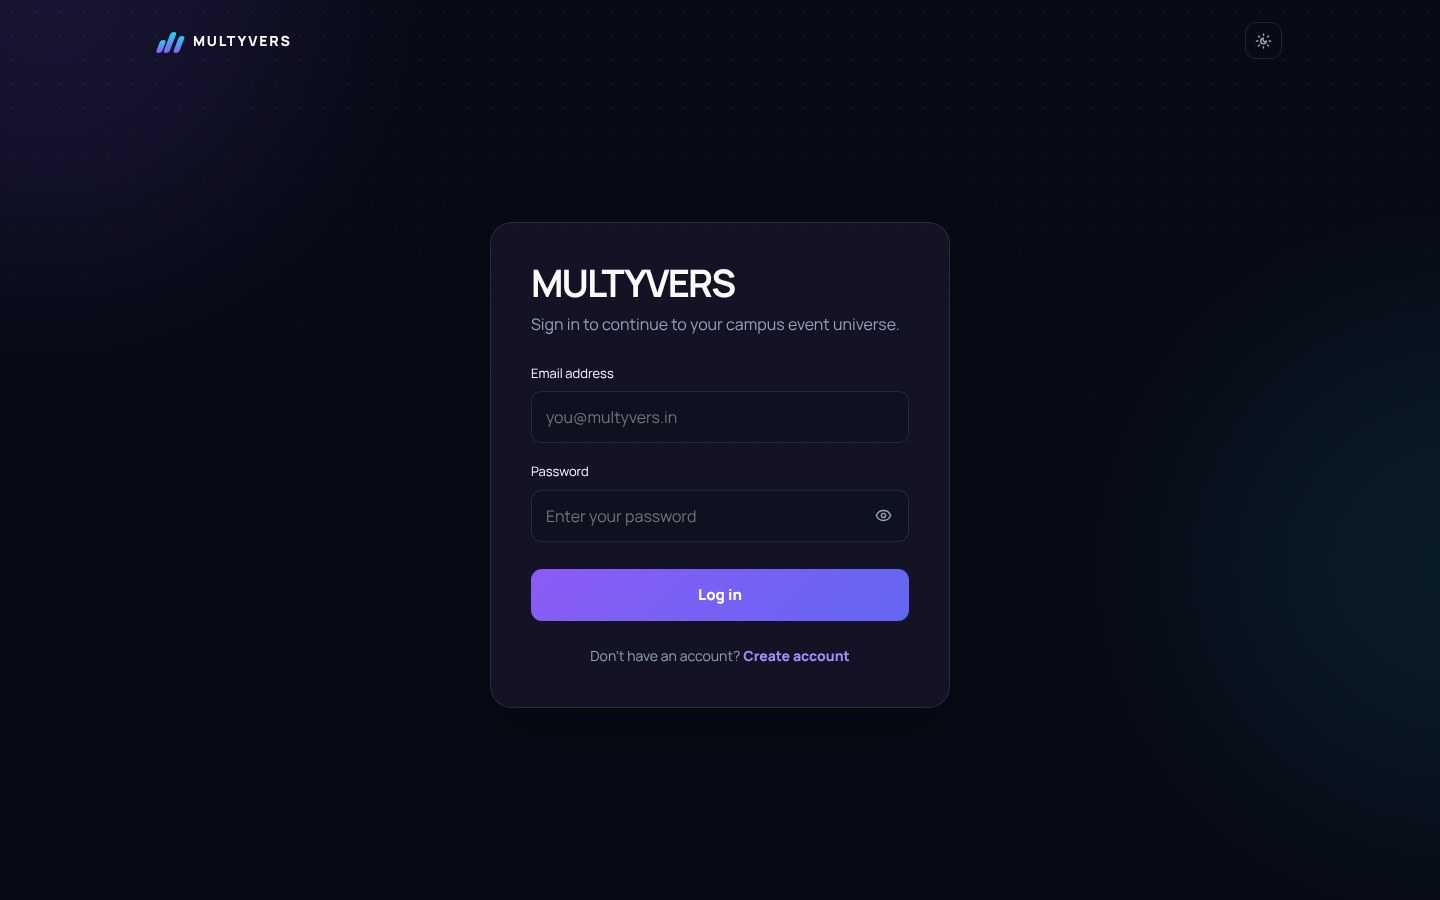
\includegraphics[width=\linewidth]{figures/screens/01_login.jpg}
\caption{Login page, the entry point of all three portals.}\label{fig:login}
\end{subfigure}\hfill
\begin{subfigure}[t]{0.485\textwidth}
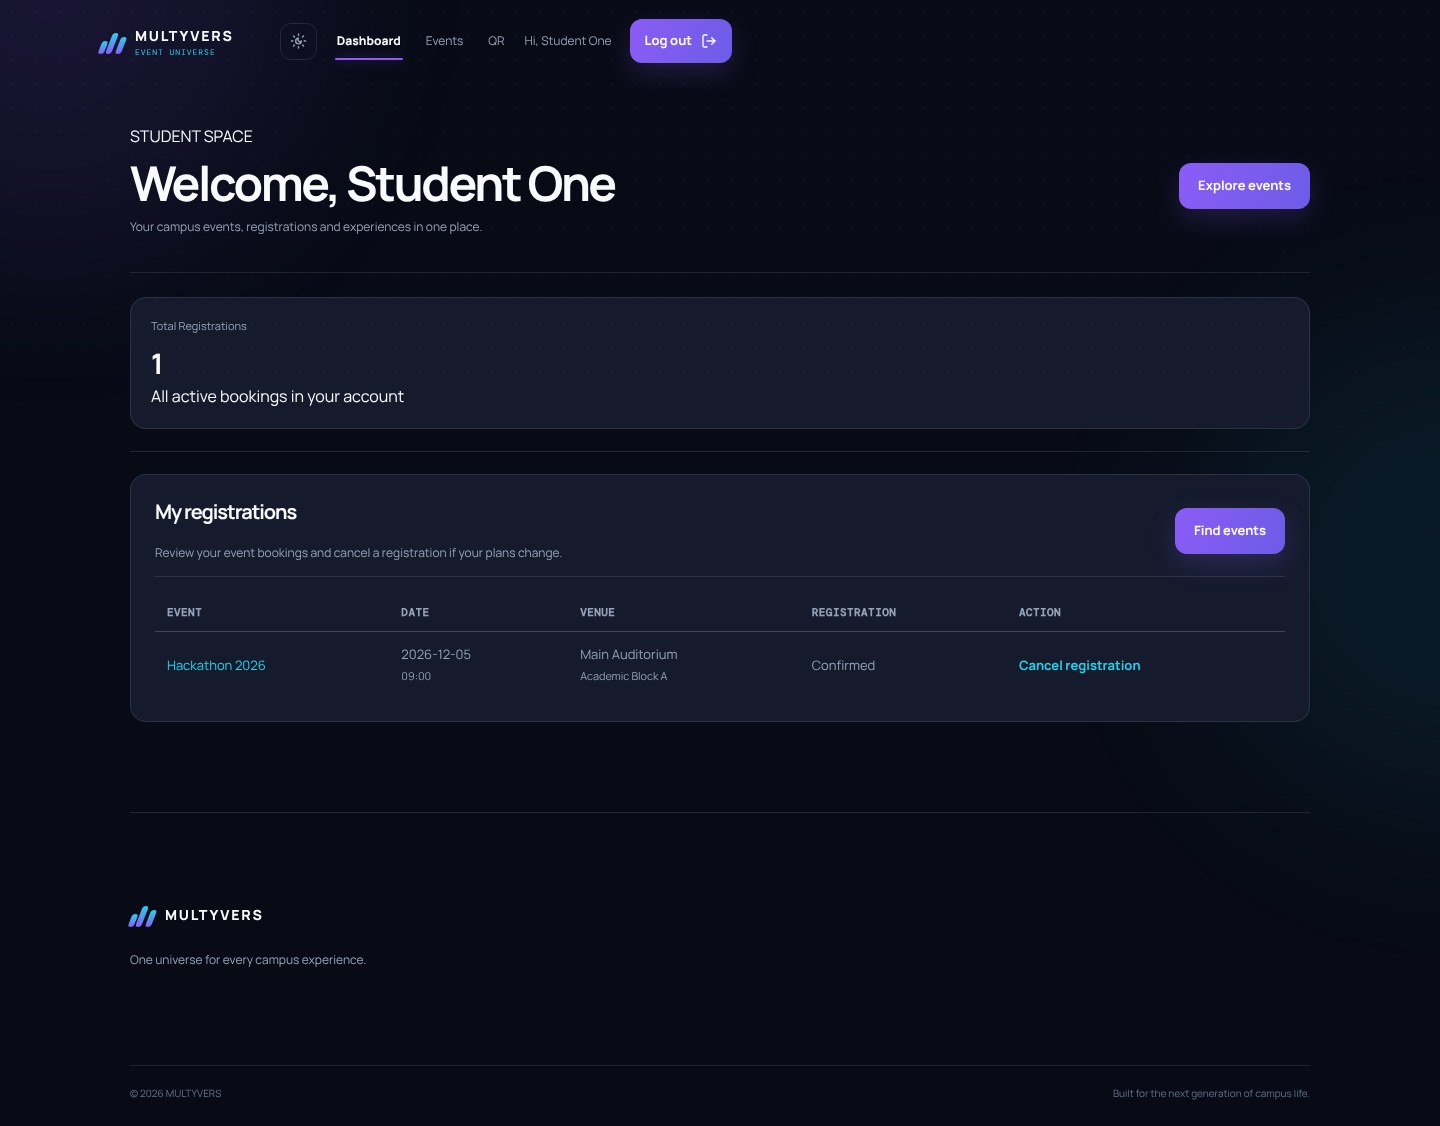
\includegraphics[width=\linewidth]{figures/screens/04_student_dashboard.jpg}
\caption{Student dashboard with the registration and cancel action.}\label{fig:sdash}
\end{subfigure}
\caption{Login and student dashboard.}
\end{figure}

\begin{figure}[H]
\centering
\begin{subfigure}[t]{0.485\textwidth}
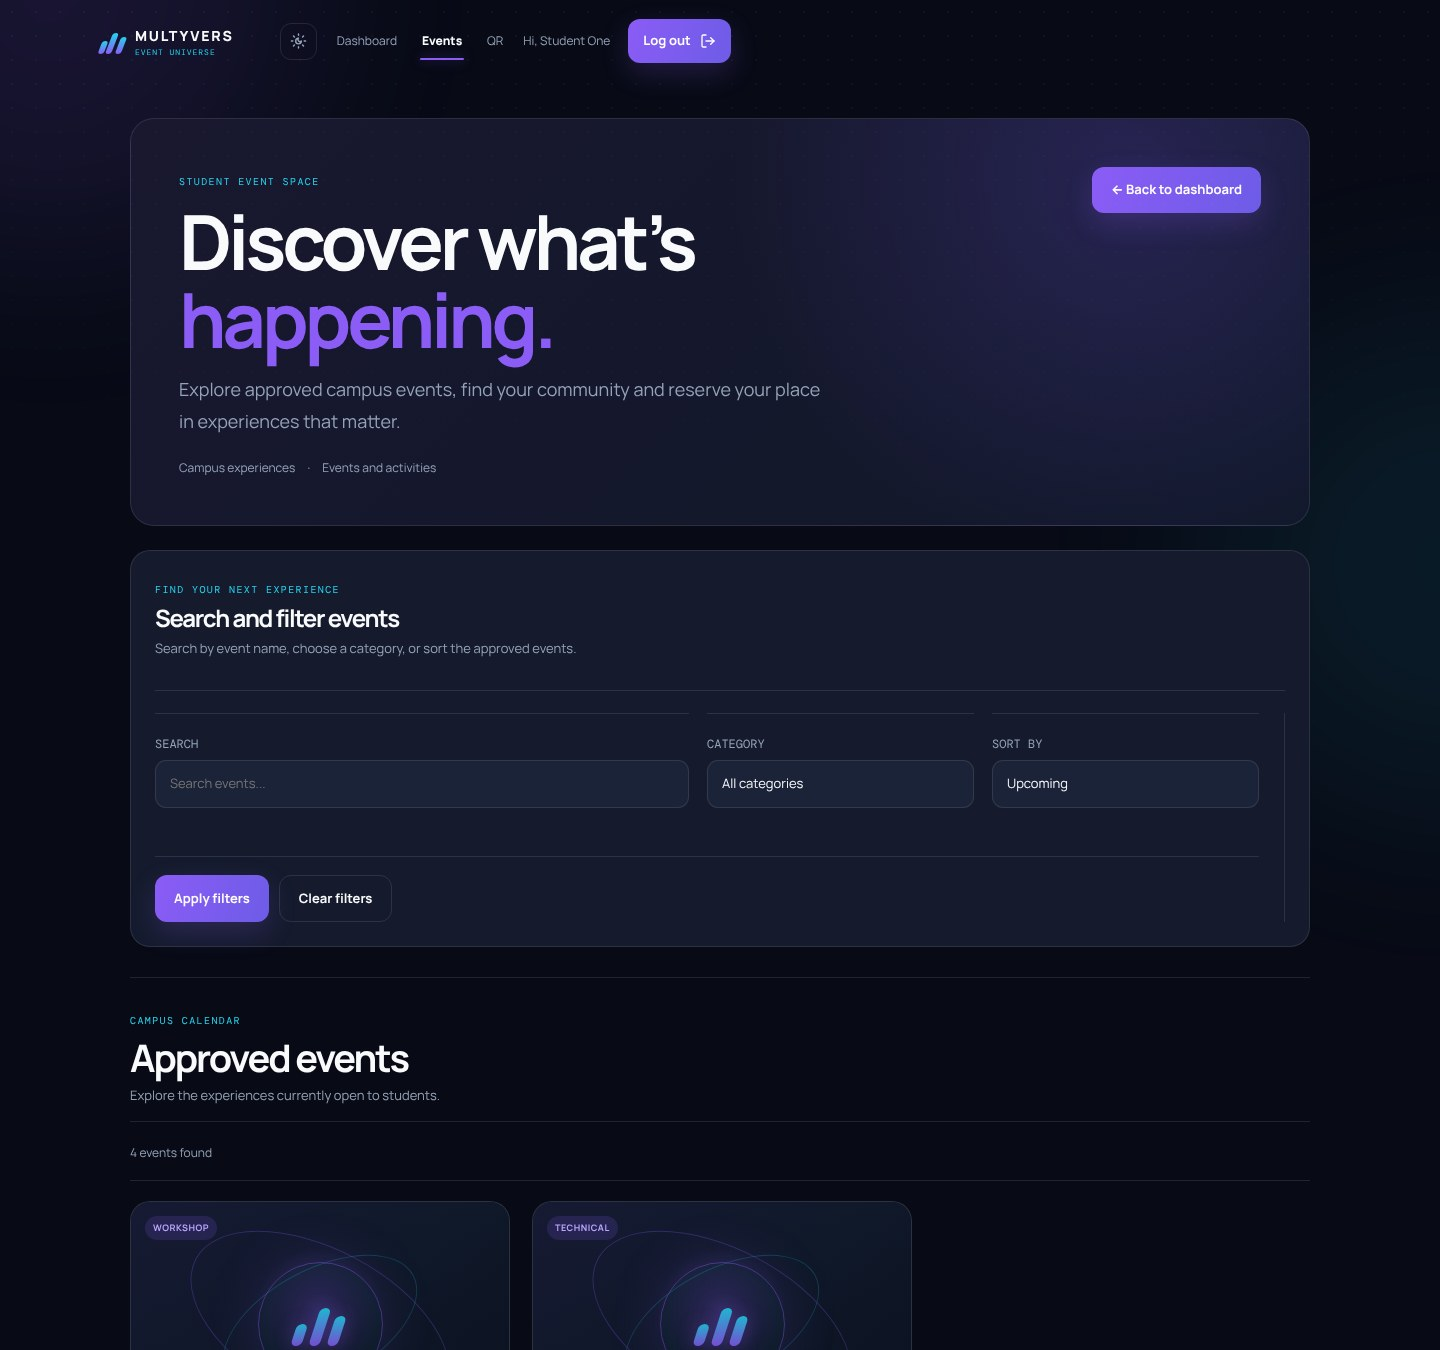
\includegraphics[width=\linewidth]{figures/screens/05_event_listing.jpg}
\caption{Event listing with search, category filter and sorting (cropped).}\label{fig:events}
\end{subfigure}\hfill
\begin{subfigure}[t]{0.485\textwidth}
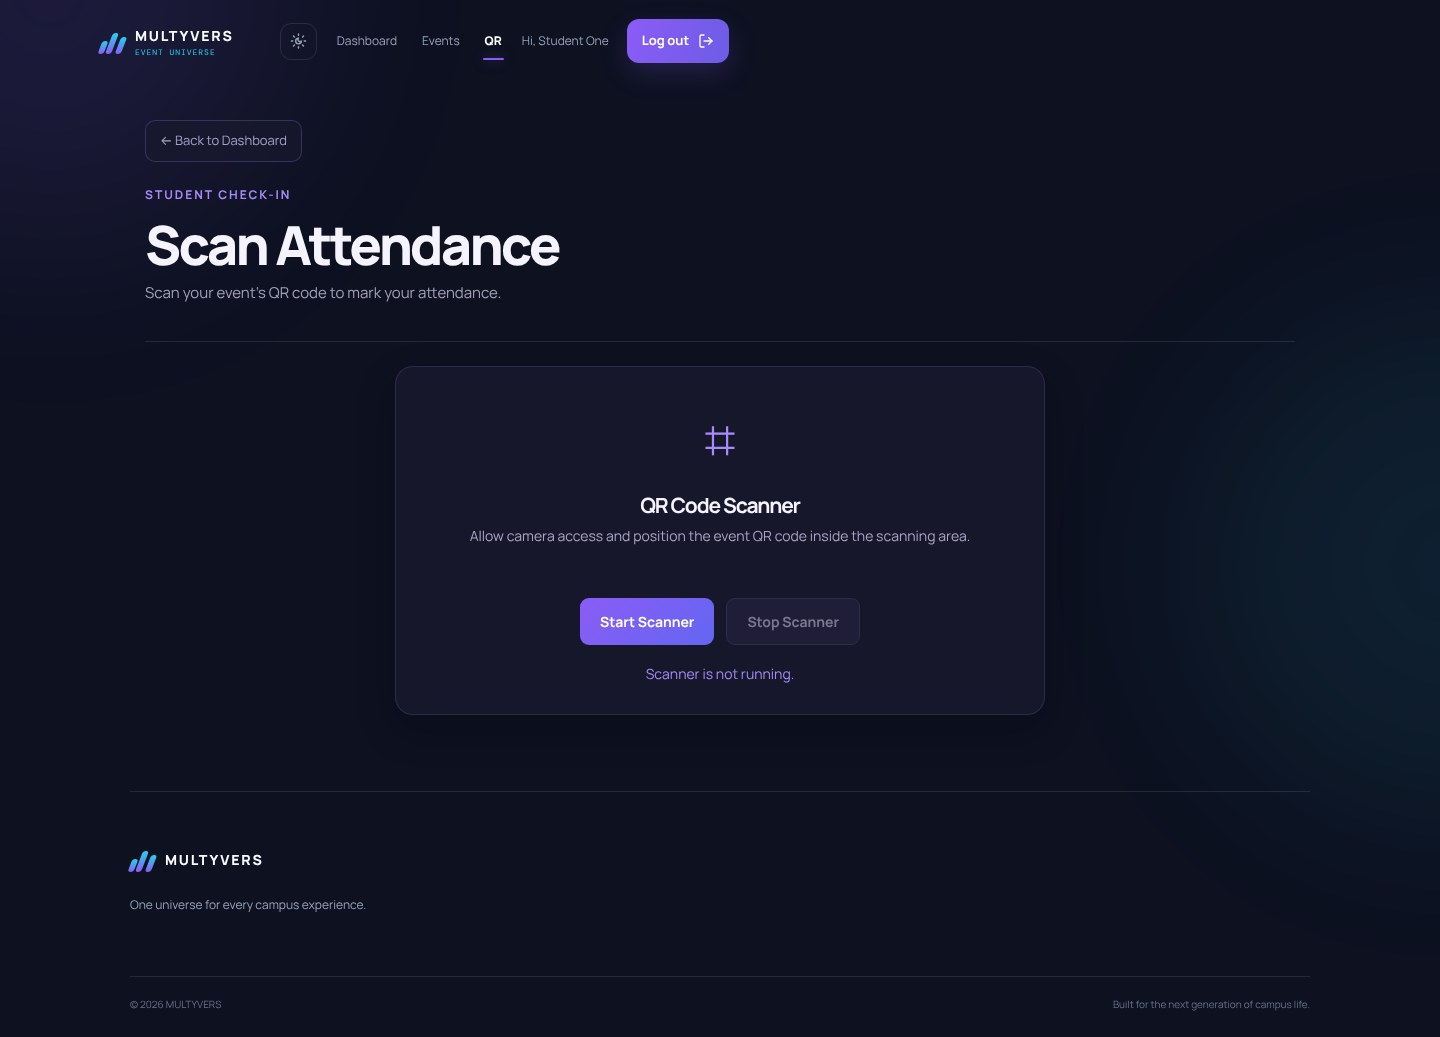
\includegraphics[width=\linewidth]{figures/screens/08_student_qr_scanner.jpg}
\caption{Student attendance page with the QR scanner (idle state).}\label{fig:scanner}
\end{subfigure}
\caption{Event discovery and the attendance scanner page.}
\end{figure}

\begin{figure}[H]
\centering
\begin{subfigure}[t]{0.485\textwidth}
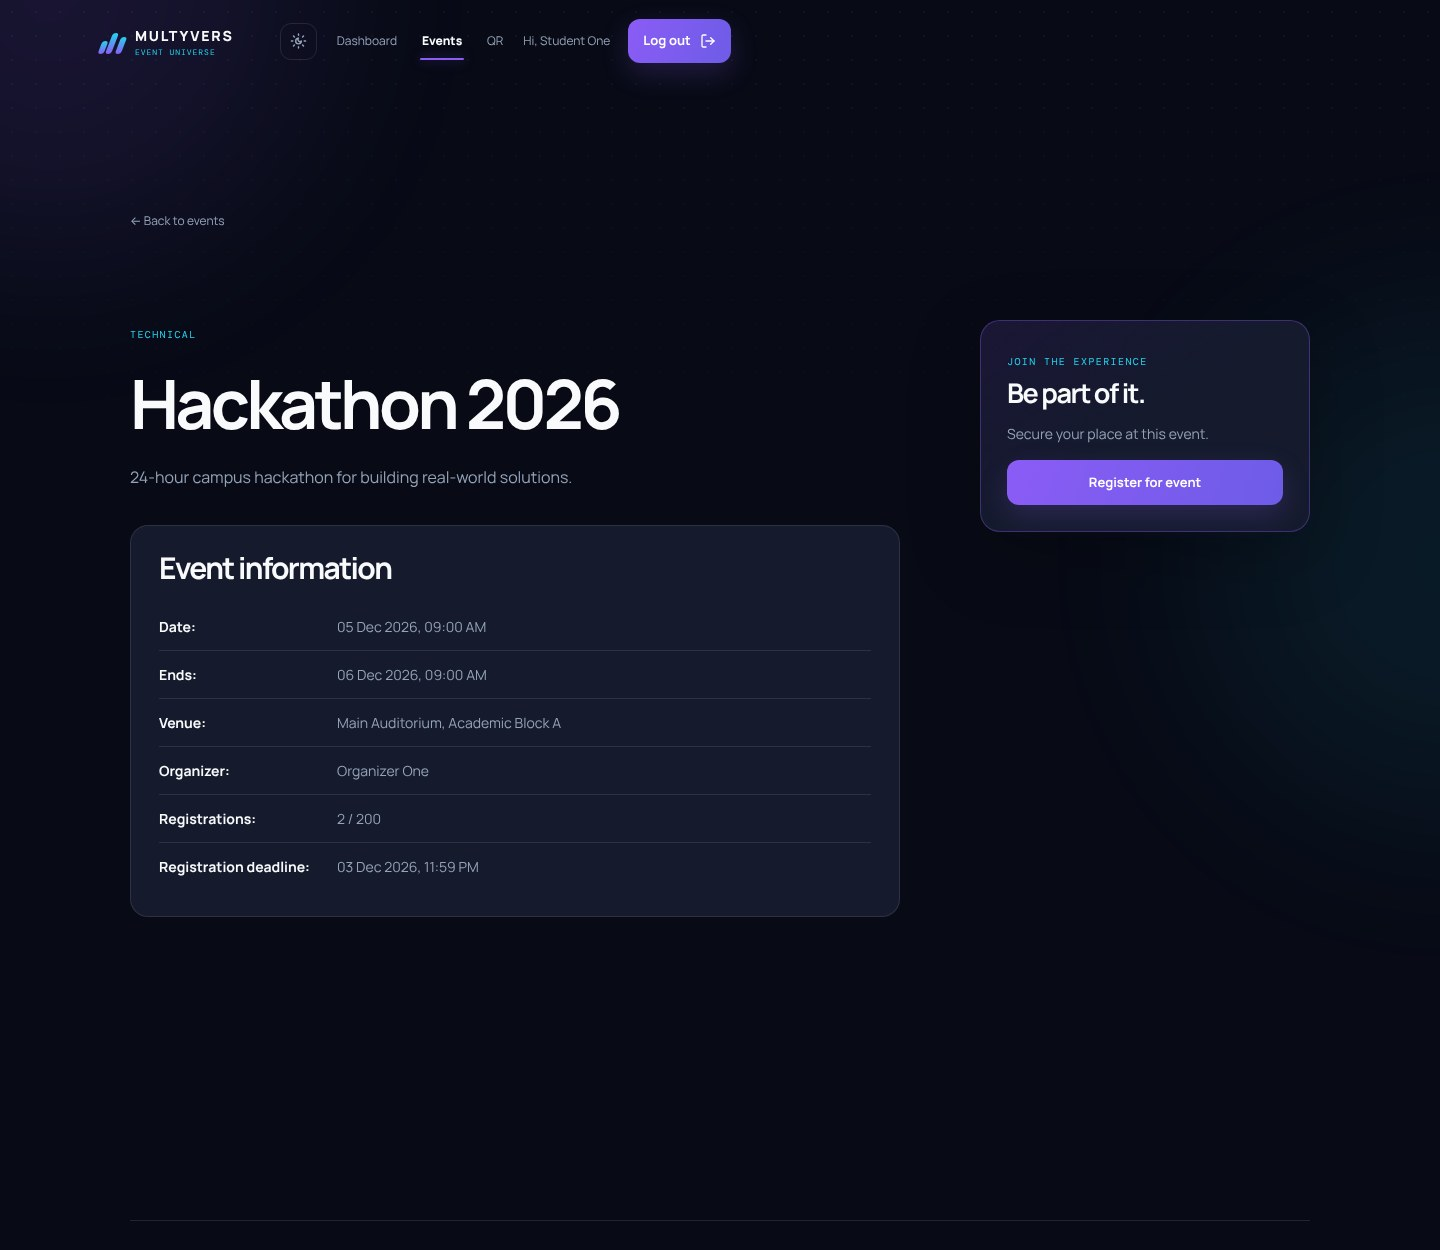
\includegraphics[width=\linewidth]{figures/screens/06_event_detail_before_registration.jpg}
\caption{Before registering.}\label{fig:detail-a}
\end{subfigure}\hfill
\begin{subfigure}[t]{0.485\textwidth}
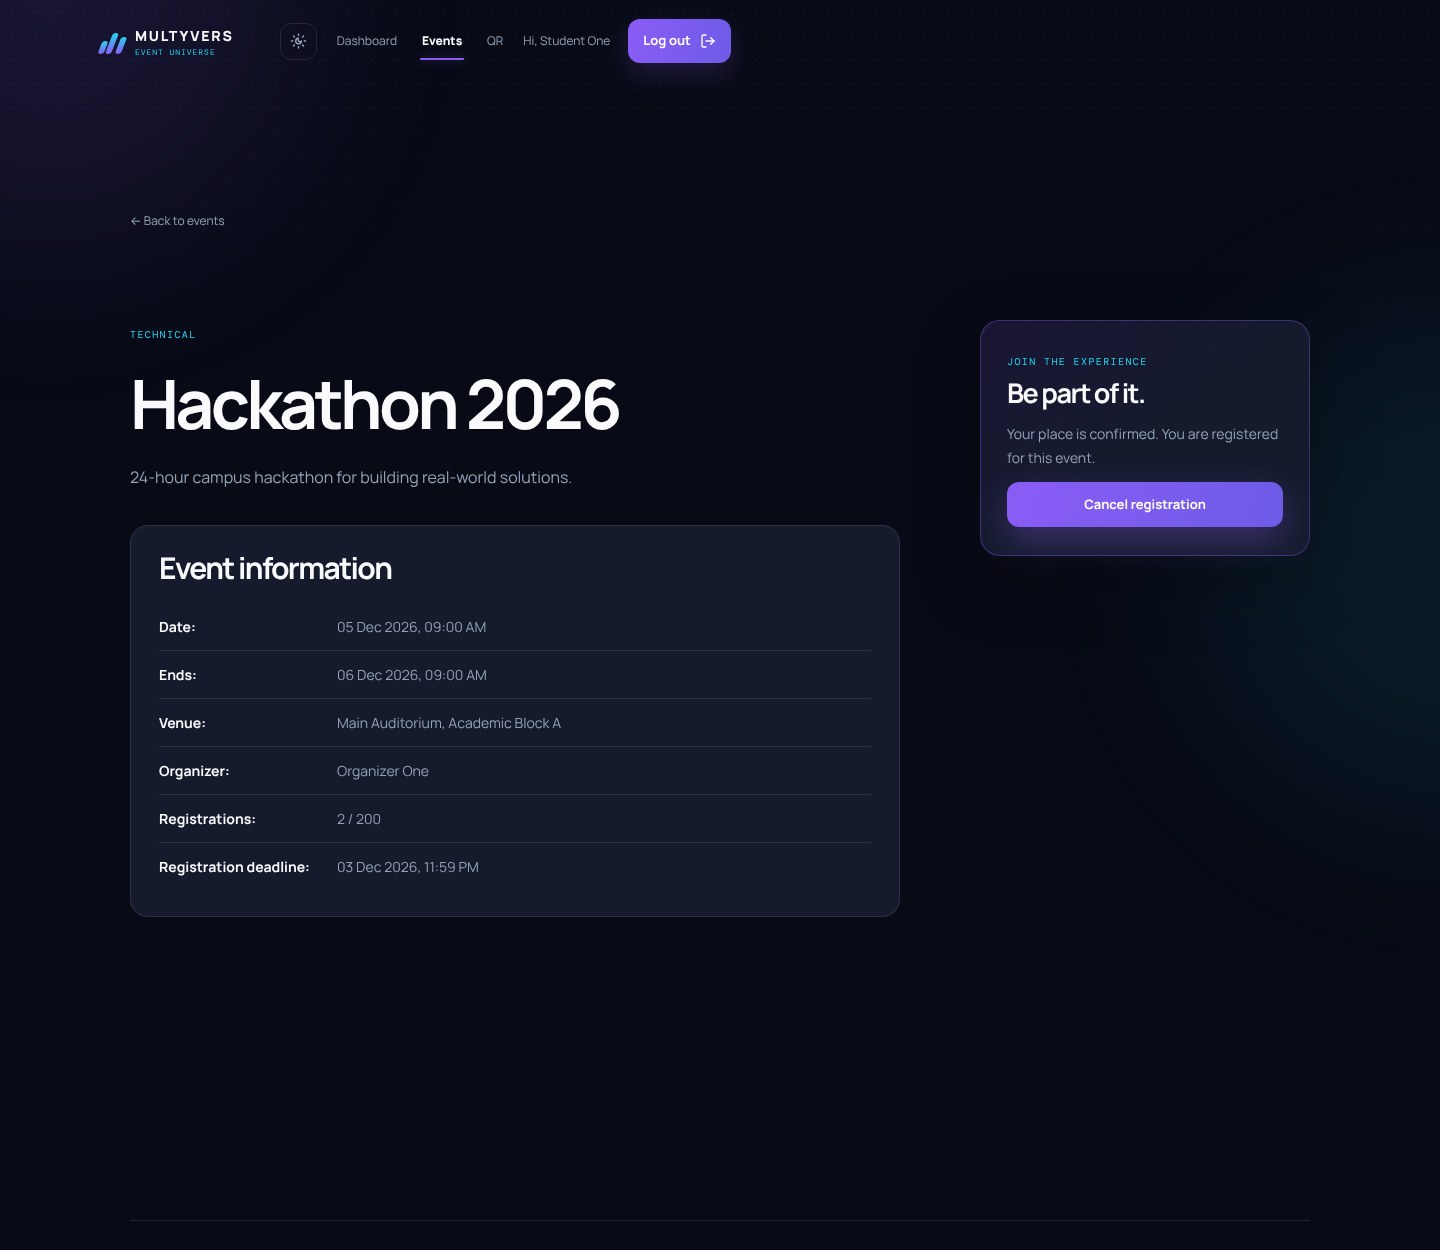
\includegraphics[width=\linewidth]{figures/screens/07_event_registered.jpg}
\caption{After registering: confirmed, with cancel option.}\label{fig:detail-b}
\end{subfigure}
\caption{Event detail page and registration.}
\label{fig:detail}
\end{figure}

\subsection{Organizer portal}
After approval, an organizer starts from the dashboard (Figure~\ref{fig:odash}) and creates an event with the form in
Figure~\ref{fig:create}, which includes the venue availability checker. Participants are reviewed in Figure~\ref{fig:participants}, where
the attendance of each participant is visible. Figure~\ref{fig:attendance} shows the QR code generated for an event that was running
at the time, and the attendance report below it with one student checked in through the real attendance endpoint. The analytics
dashboard is shown in Figure~\ref{fig:analytics}.

\begin{figure}[H]
\centering
\begin{subfigure}[t]{0.485\textwidth}
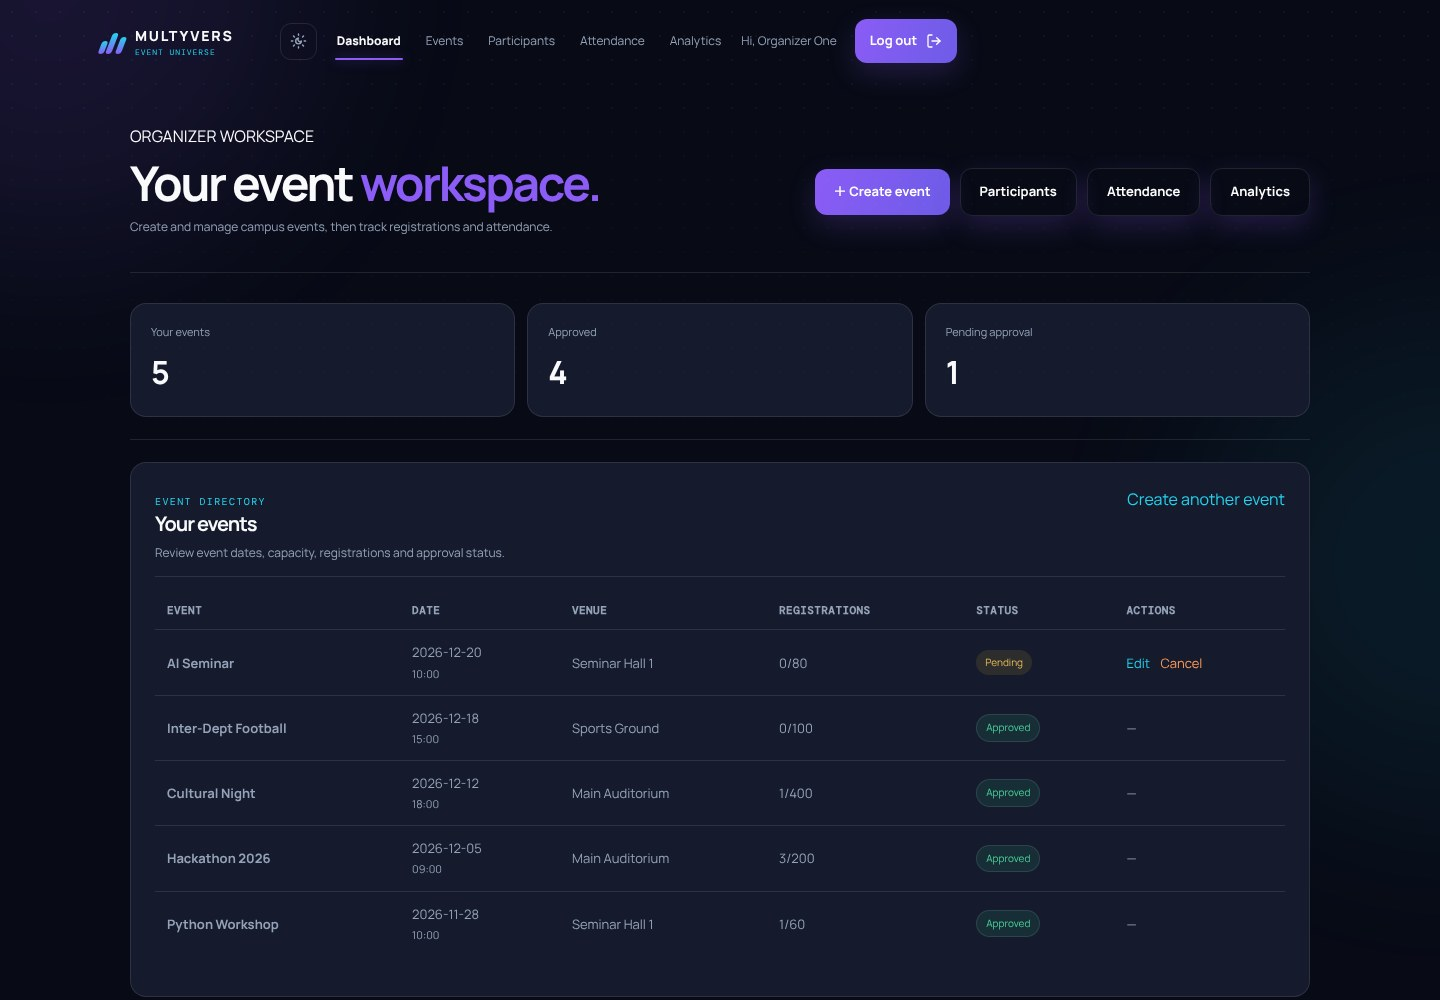
\includegraphics[width=\linewidth]{figures/screens/09_organizer_dashboard.jpg}
\caption{Organizer dashboard: counts and own events (cropped).}\label{fig:odash}
\end{subfigure}\hfill
\begin{subfigure}[t]{0.485\textwidth}
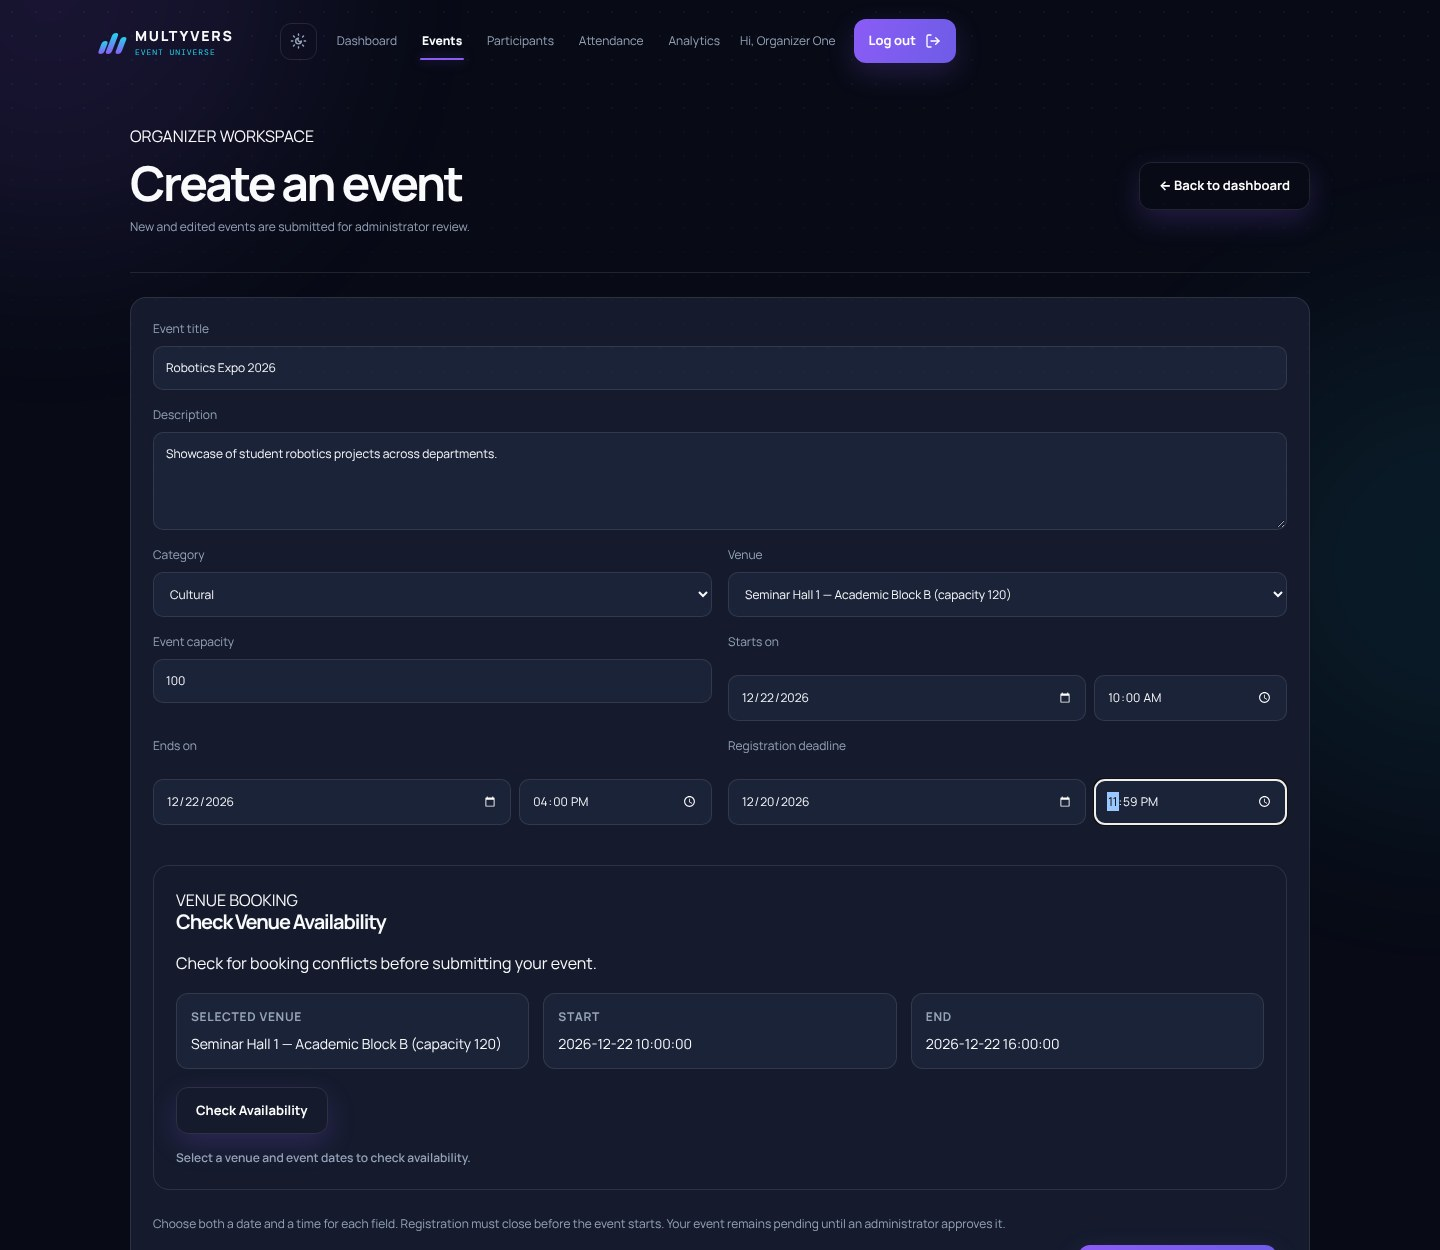
\includegraphics[width=\linewidth]{figures/screens/10_organizer_event_creation.jpg}
\caption{Event creation form (filled in, not submitted).}\label{fig:create}
\end{subfigure}
\caption{Organizer dashboard and event creation.}
\end{figure}

\begin{figure}[H]
\centering
\begin{subfigure}[t]{0.485\textwidth}
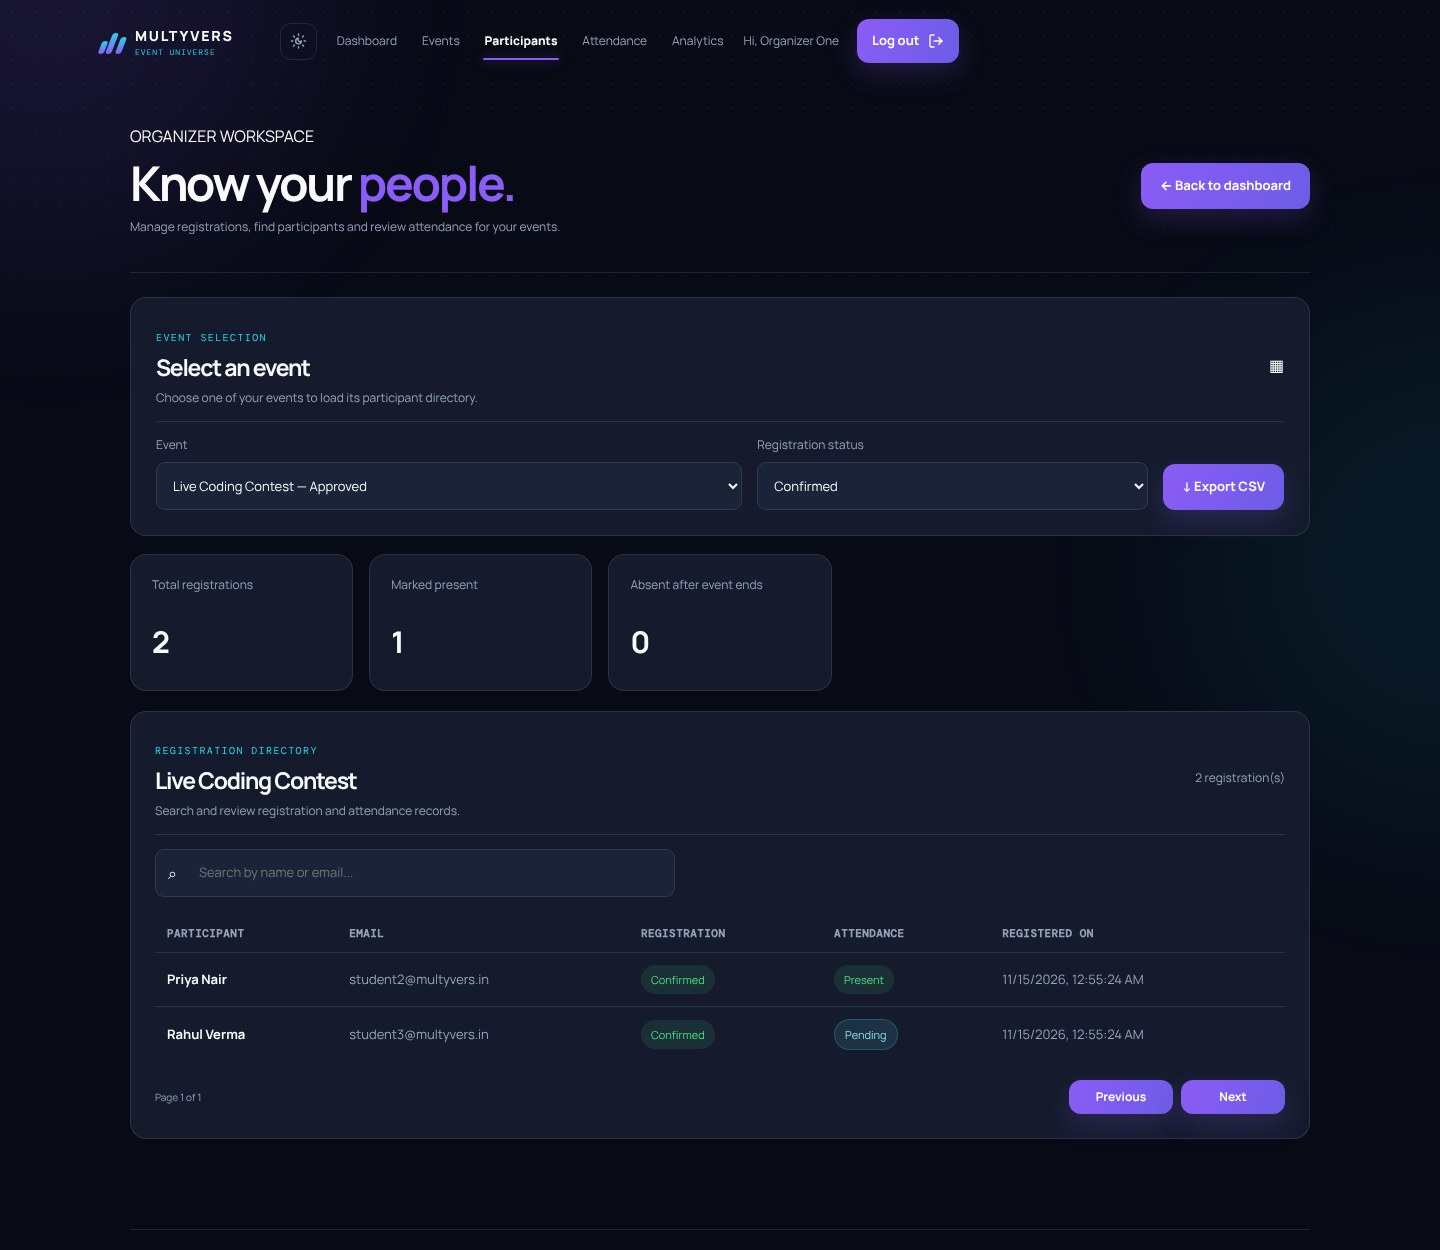
\includegraphics[width=\linewidth]{figures/screens/11_organizer_participants.jpg}
\caption{Participant management with registration and attendance status.}\label{fig:participants}
\end{subfigure}\hfill
\begin{subfigure}[t]{0.485\textwidth}
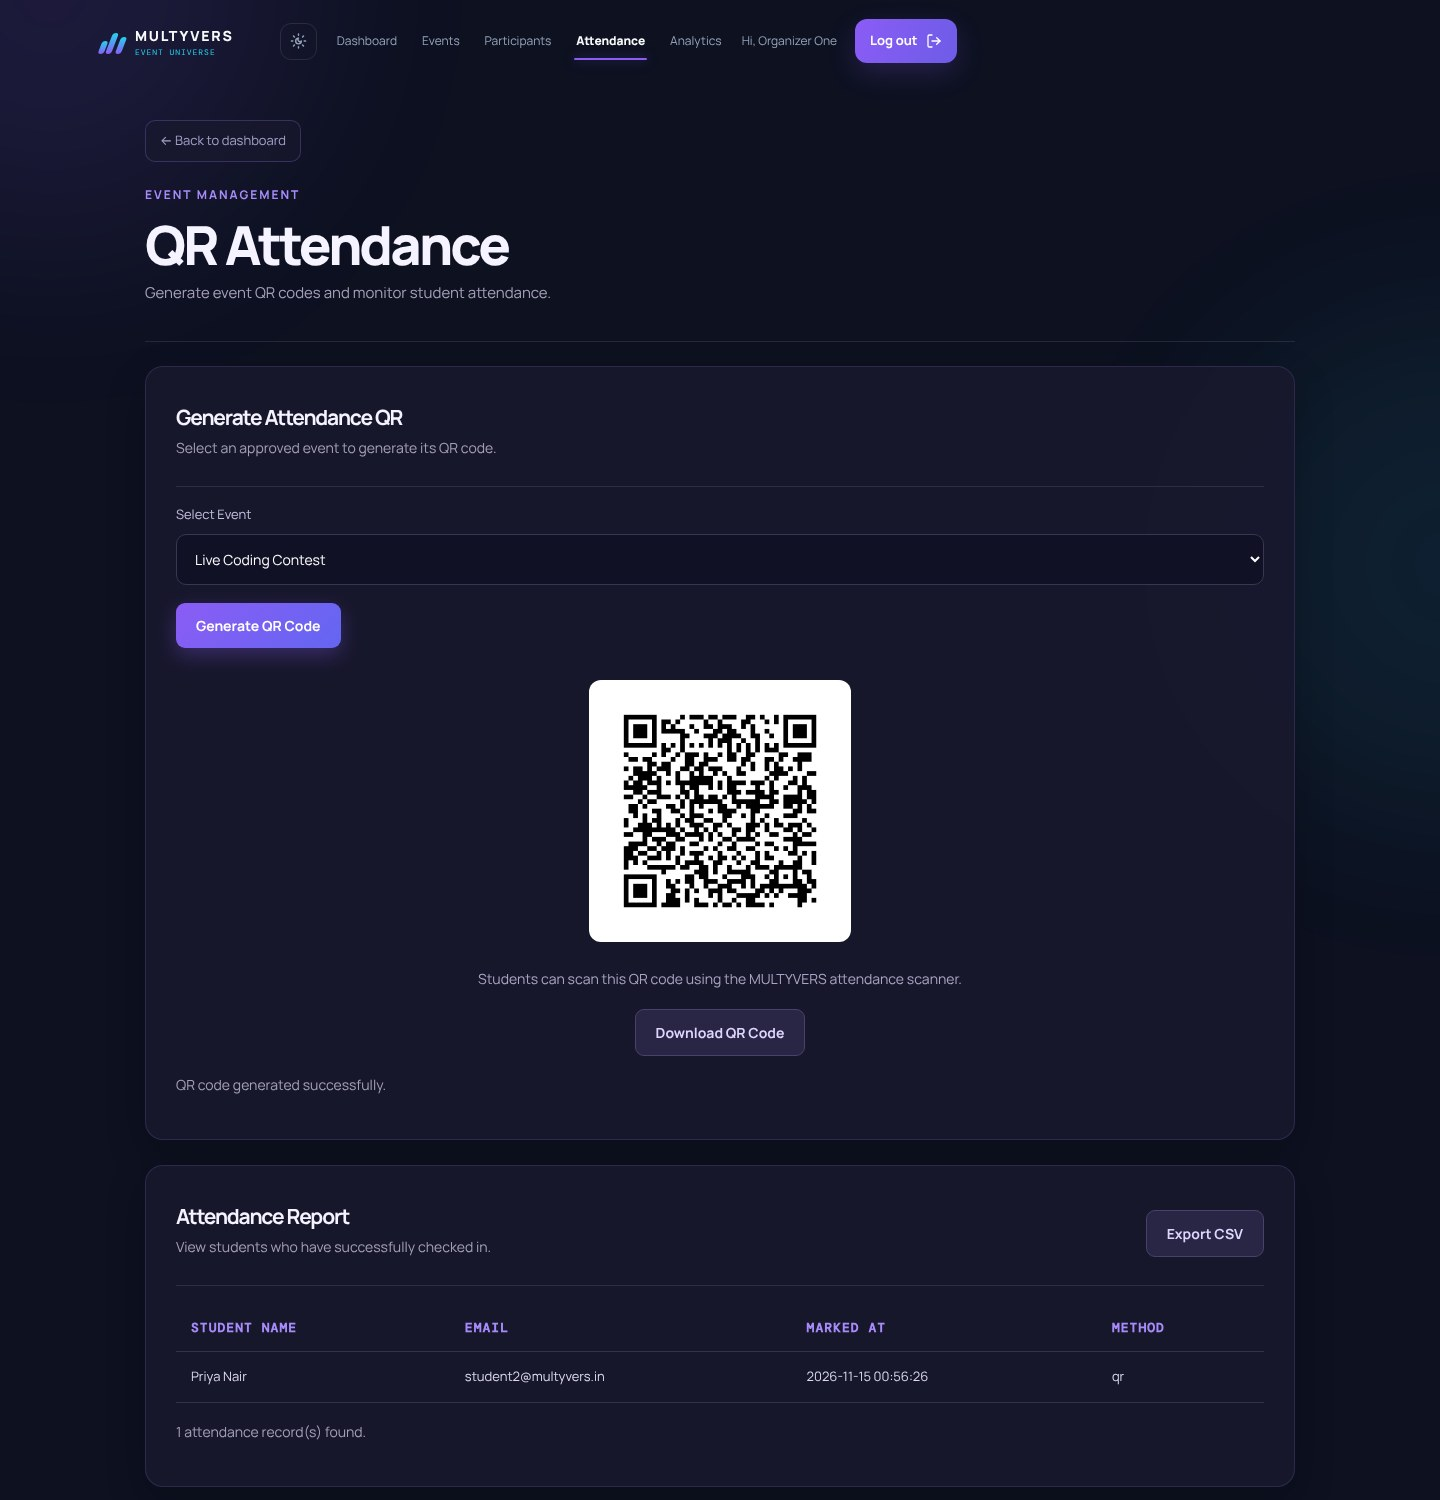
\includegraphics[width=\linewidth]{figures/screens/12_organizer_qr_attendance.jpg}
\caption{Generated QR code and attendance report.}\label{fig:attendance}
\end{subfigure}
\caption{Participants and QR attendance.}
\end{figure}

\begin{figure}[H]
\centering
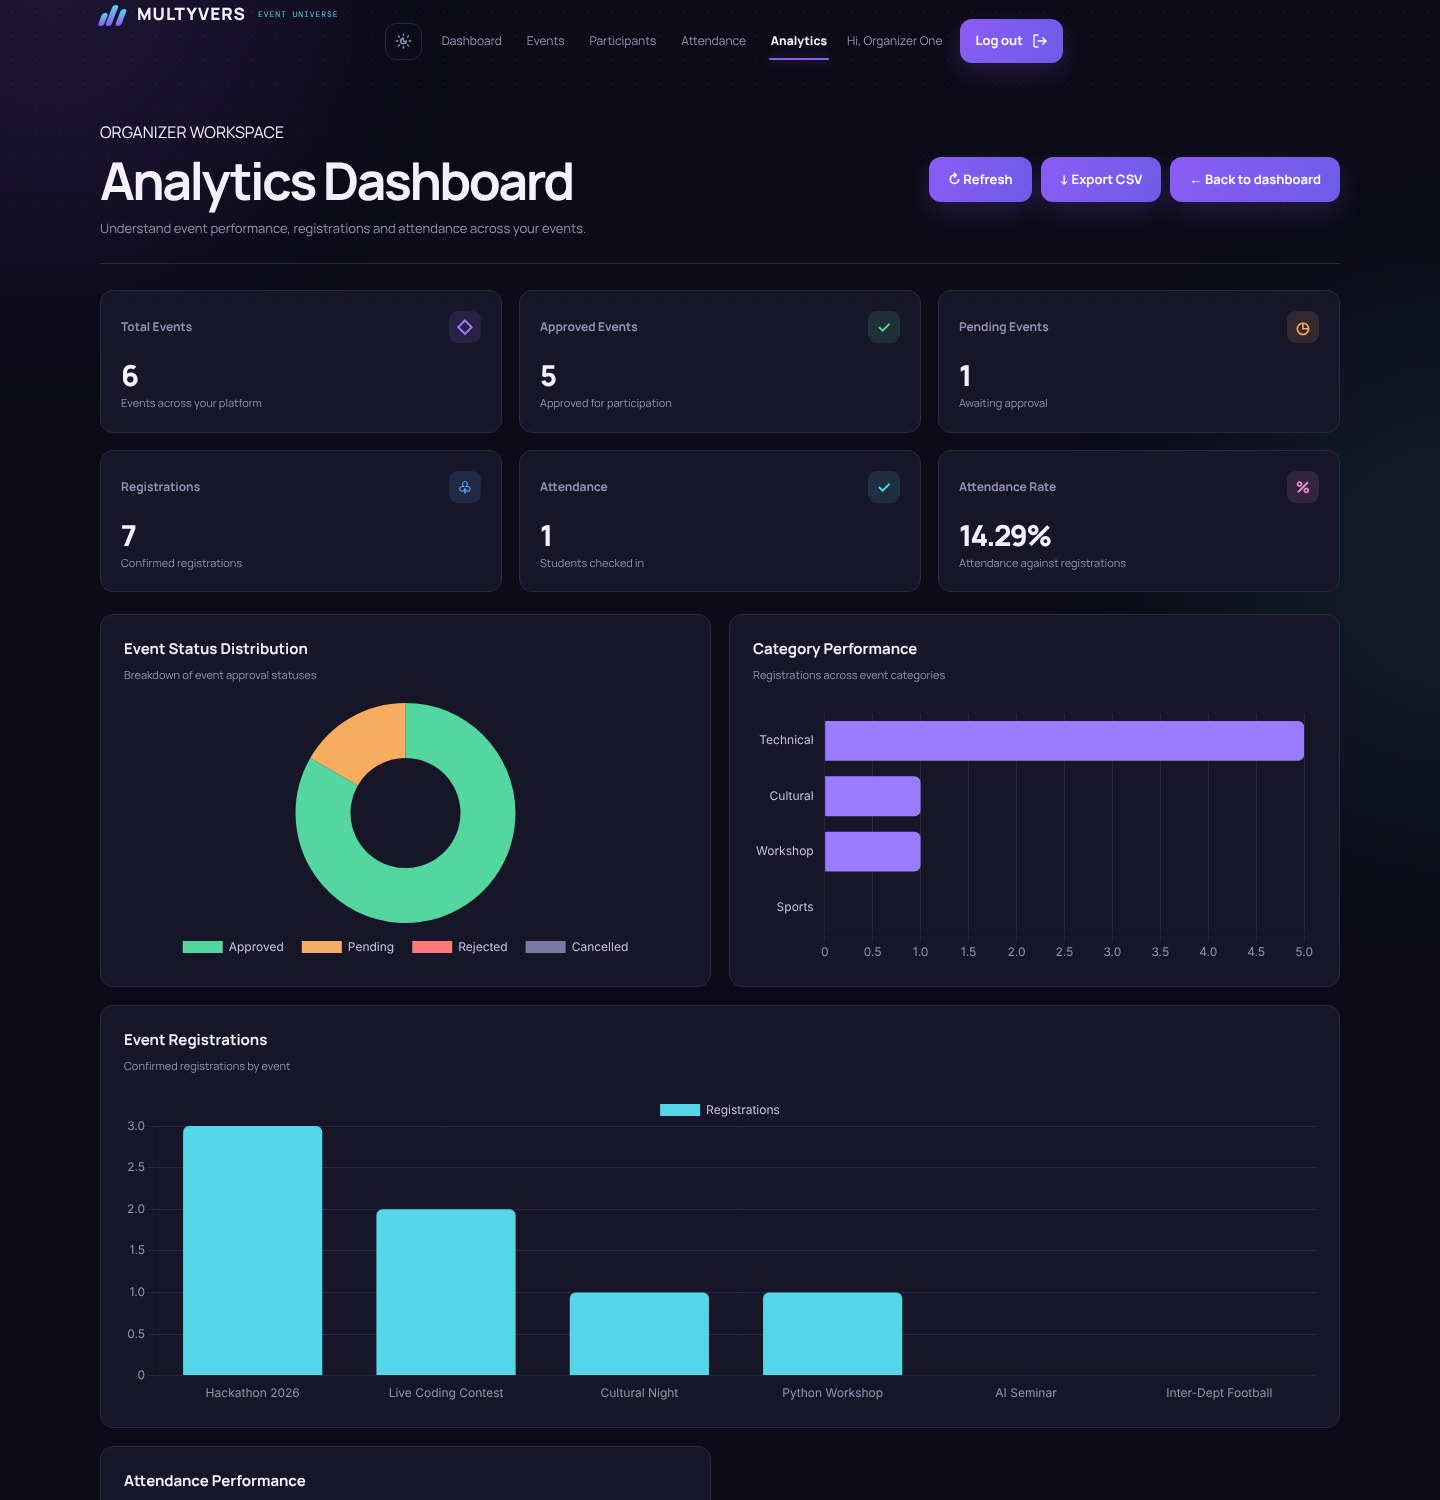
\includegraphics[width=0.6\textwidth]{figures/screens/13_organizer_analytics.jpg}
\caption{Analytics dashboard with summary cards and Chart.js charts (cropped).}
\label{fig:analytics}
\end{figure}

\subsection{Admin portal}
The admin dashboard (Figure~\ref{fig:adash}) summarises users, organizers, pending requests and events. Pending organizer requests are approved or
rejected in Figure~\ref{fig:aorg} and pending events in Figure~\ref{fig:aevent}. Venues (Figure~\ref{fig:avenue}), categories
(Figure~\ref{fig:acat}) and student accounts (Figure~\ref{fig:astud}) are maintained on their own pages.

\begin{figure}[H]
\centering
\begin{subfigure}[t]{0.485\textwidth}
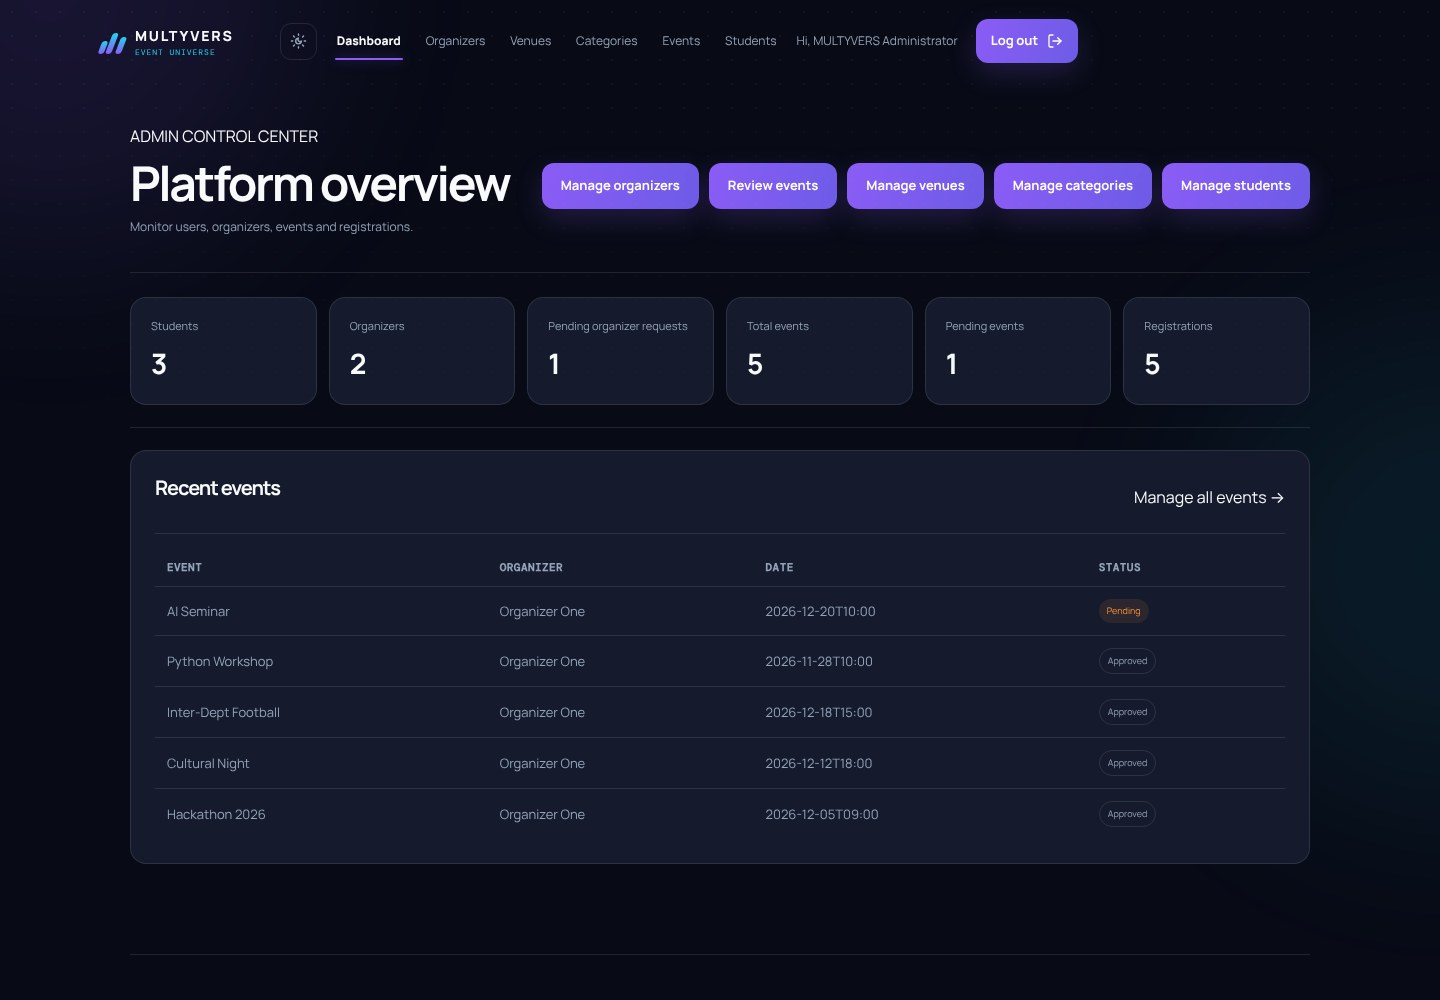
\includegraphics[width=\linewidth]{figures/screens/14_admin_dashboard.jpg}
\caption{Admin dashboard (platform overview, cropped).}\label{fig:adash}
\end{subfigure}\hfill
\begin{subfigure}[t]{0.485\textwidth}
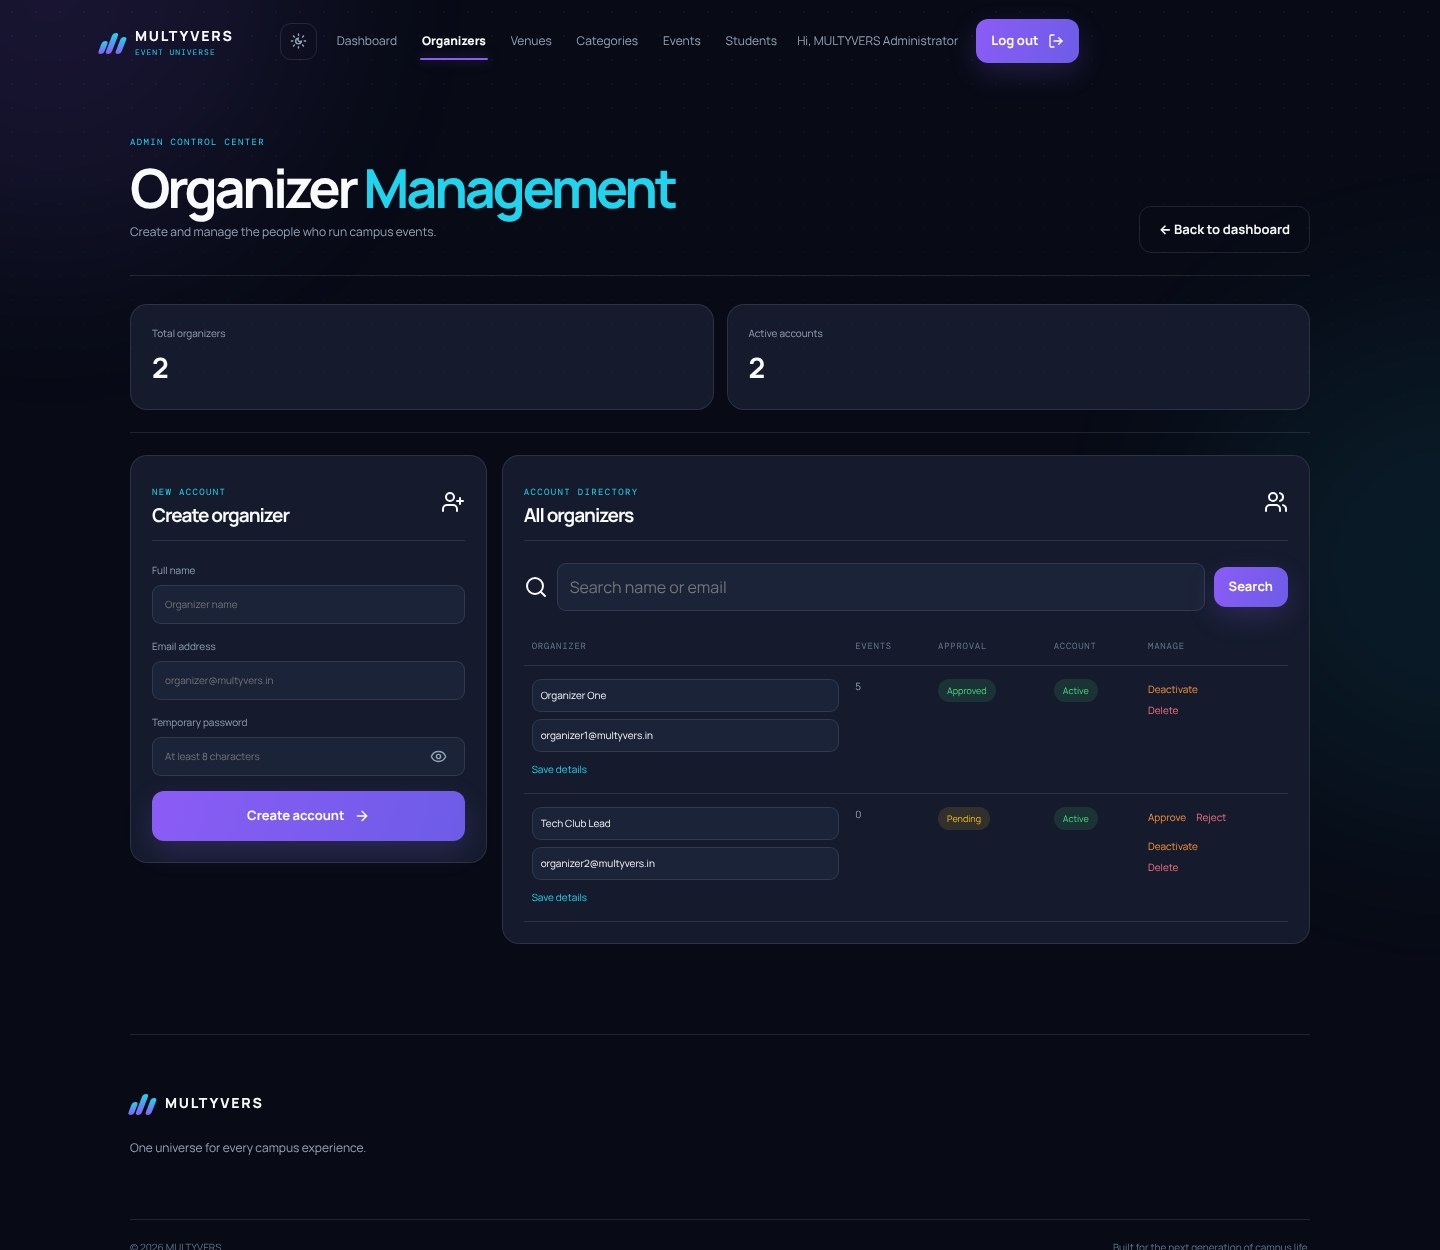
\includegraphics[width=\linewidth]{figures/screens/15_admin_organizer_approval.jpg}
\caption{Organizer management: one request is pending (Approve / Reject).}\label{fig:aorg}
\end{subfigure}
\caption{Admin dashboard and organizer approval.}
\end{figure}

\begin{figure}[H]
\centering
\begin{subfigure}[t]{0.485\textwidth}
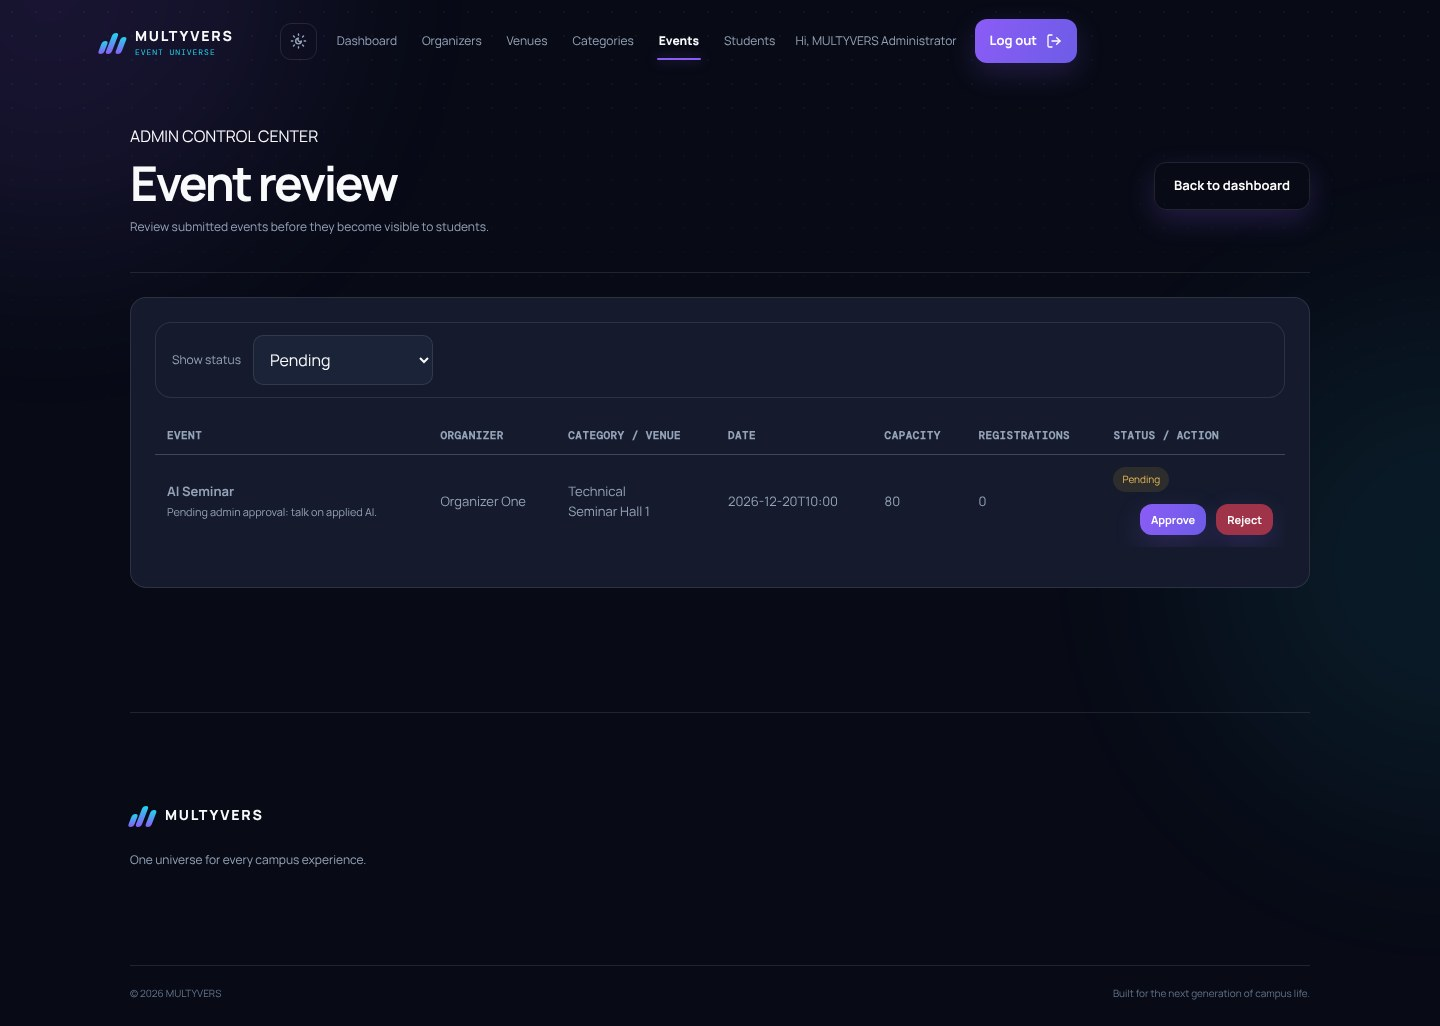
\includegraphics[width=\linewidth]{figures/screens/16_admin_event_approval.jpg}
\caption{Event review: a pending event with Approve and Reject.}\label{fig:aevent}
\end{subfigure}\hfill
\begin{subfigure}[t]{0.485\textwidth}
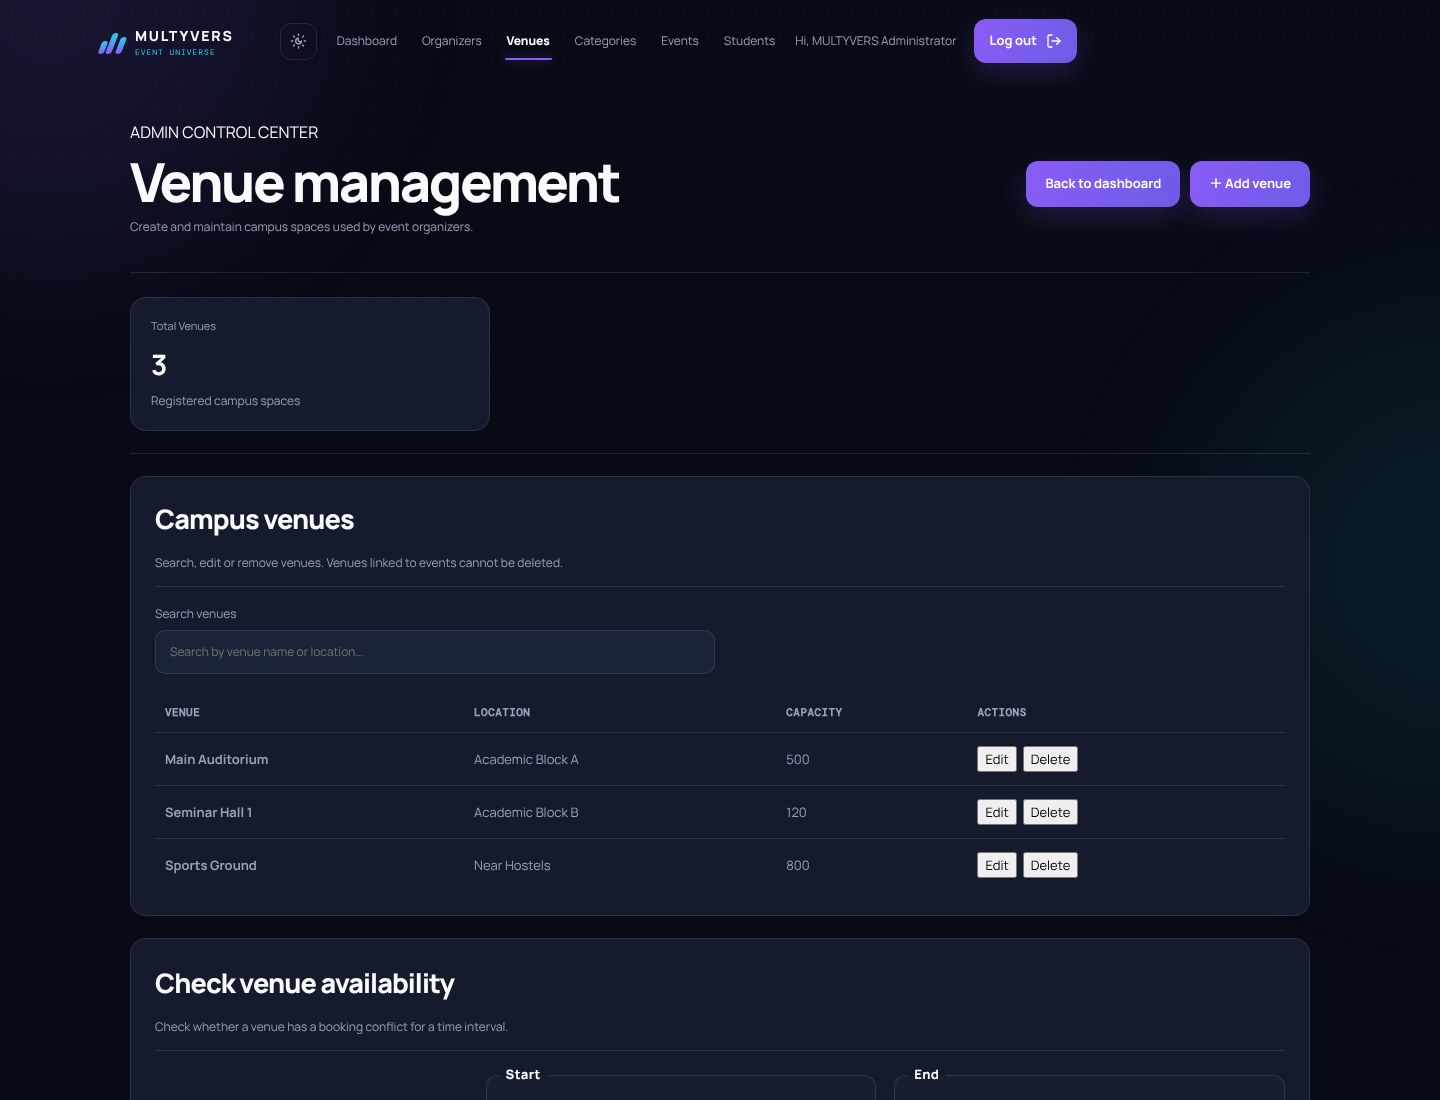
\includegraphics[width=\linewidth]{figures/screens/17_admin_venues.jpg}
\caption{Venue management with availability checker (cropped).}\label{fig:avenue}
\end{subfigure}
\caption{Event approval and venue management.}
\end{figure}

\begin{figure}[H]
\centering
\begin{subfigure}[t]{0.485\textwidth}
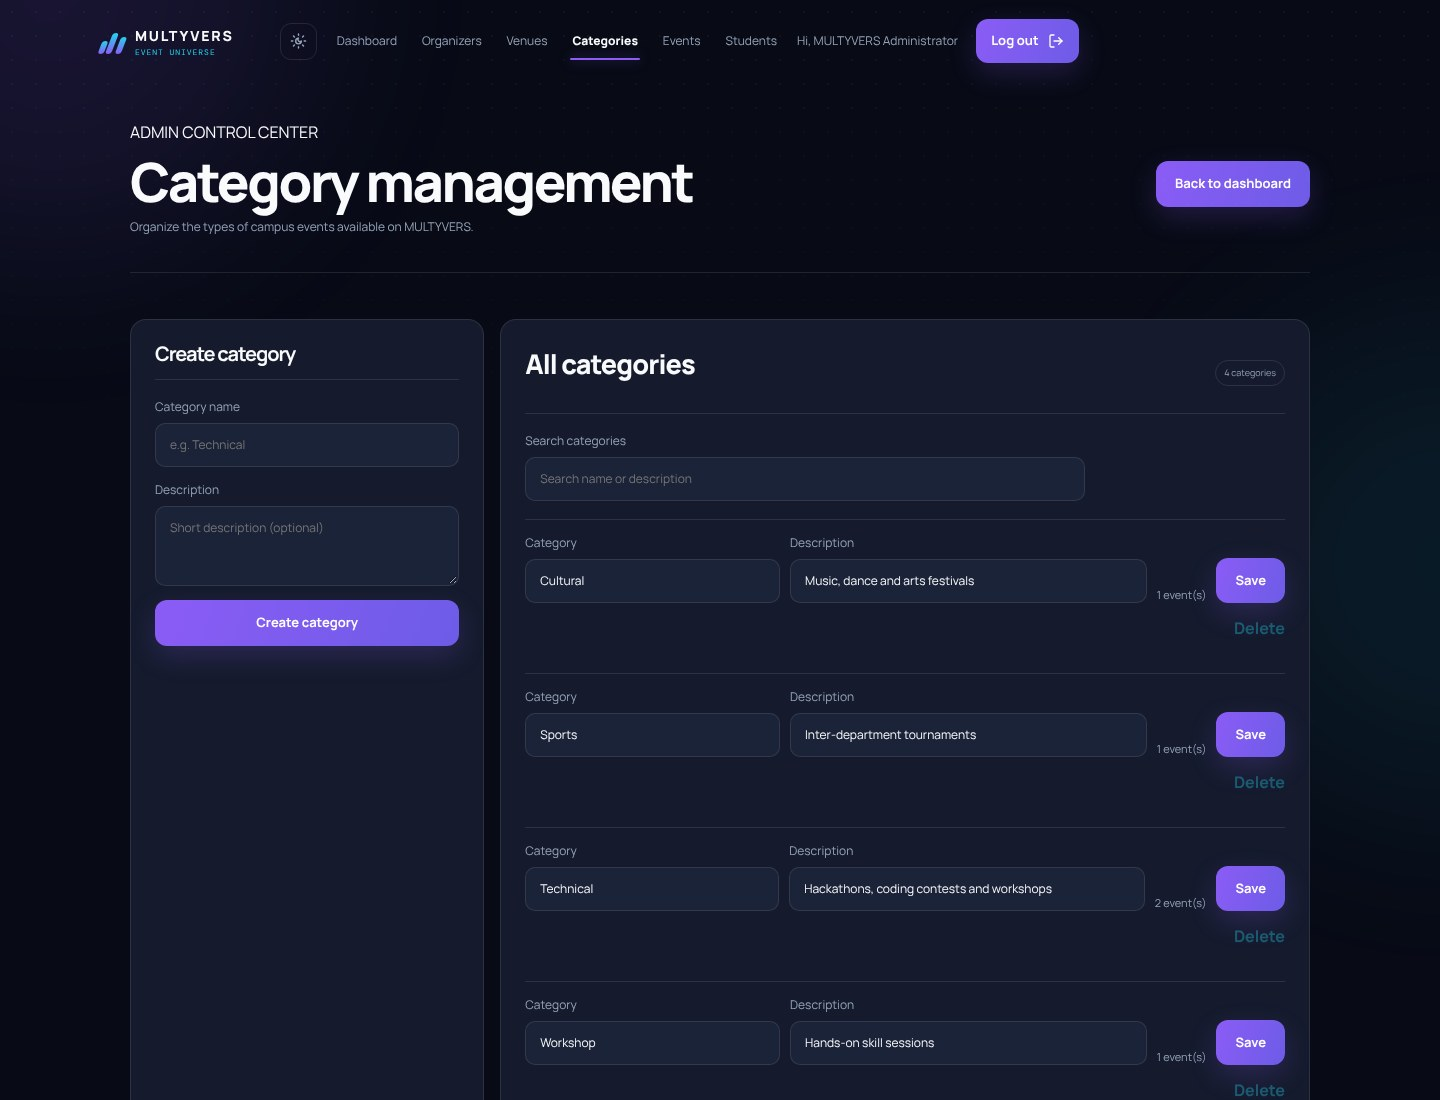
\includegraphics[width=\linewidth]{figures/screens/18_admin_categories.jpg}
\caption{Category management (cropped).}\label{fig:acat}
\end{subfigure}\hfill
\begin{subfigure}[t]{0.485\textwidth}
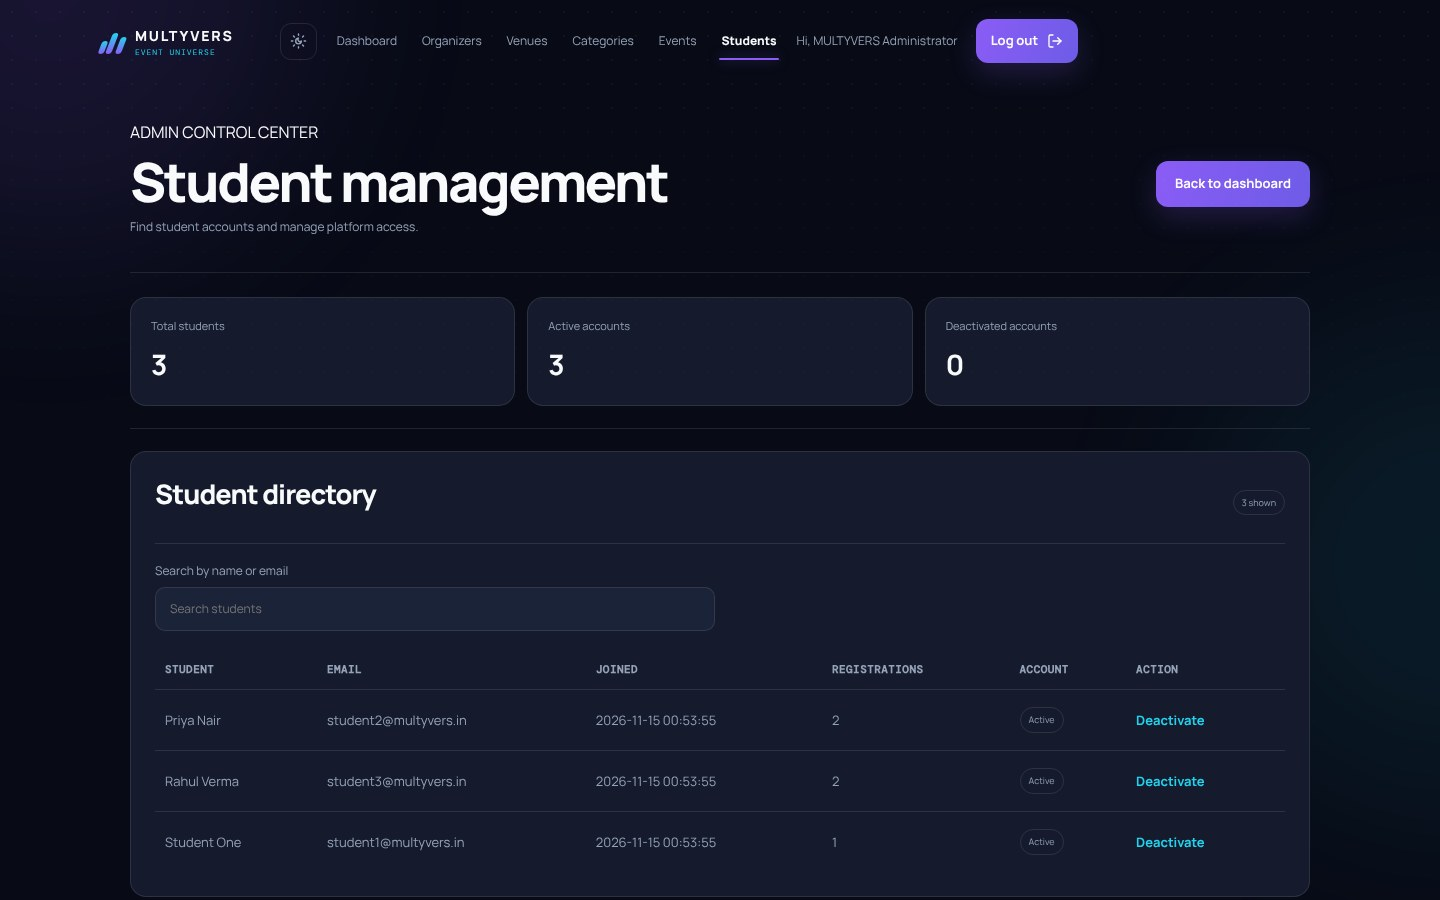
\includegraphics[width=\linewidth]{figures/screens/19_admin_students.jpg}
\caption{Student management.}\label{fig:astud}
\end{subfigure}
\caption{Category and student management.}
\end{figure}

% ================= 10 CONCLUSION =================
\section{Conclusion}
\label{sec:conclusion}

\subsection{What MULTYVERS achieves}
MULTYVERS replaces the separate steps of campus event management with one application. An organizer proposes an event with a venue, the administrator approves it after
checking for venue clashes, students register within capacity and deadline, and on the day attendance is recorded through a signed QR code and reported back to the organizer
together with analytics. The three portals share one database and one set of rules, which is what keeps them consistent: a registration made in the student portal is immediately the participant seen
by the organizer and a count on the administrator's overview. The 222 functional tests give confidence that the rules on roles, registration, venues and attendance hold.

Through the project we gained practice in structuring a Flask application into blueprints, designing a relational schema with constraints, writing server-side validation and
transactions, building templates and CSS for several user interfaces, testing with pytest and temporary databases, working with Git branches and merges, and documenting in \LaTeX{}.

% ================= REFERENCES =================
\bibliographystyle{plainnat}
\bibliography{references}
\addcontentsline{toc}{section}{References}

% ================= AI USE DECLARATION =================
\clearpage
\section*{AI Use Declaration}
\addcontentsline{toc}{section}{AI Use Declaration}

We acknowledge that artificial intelligence (AI) tools were used as assistance
during the development of MULTYVERS and in preparing parts of this report.
The AI tools assisted with generating and refining code, explaining unfamiliar
libraries and programming concepts, suggesting implementation approaches,
identifying and resolving errors, and helping with documentation.

The project requirements, intended features, overall user journey, and the
way the different parts of the website should be organised and connected were
directed by us. We decided what the platform should do, how the student,
organizer and administrator portals should work together, which features
should be included, and how the completed application should be arranged as
one system. We guided the use of AI tools towards these requirements and
reviewed, tested, adjusted and integrated the generated assistance into the
project.

We understand the purpose and general working of the functionality included
in the application, including the main request flow, role-based portals,
event creation and approval, registration, venue checking, participant
management, QR-based attendance, and analytics. However, we do not claim to
have mastered every library, implementation detail or line of code. Our
understanding is at the level needed to explain the features, their intended
behaviour and the main approach used; some of the newer concepts and
implementation details were learned with AI assistance and may require
further study before we can independently reproduce every part.

The code used in the project was substantially developed with AI assistance.
Our contribution was to define and guide the requirements, make decisions
about the website's structure and feature flow, direct the implementation,
review the results, make changes where needed, and bring the separate
functionalities together into the final application. The concepts and
procedures covered directly in CS202C were applied through our course
learning; additional concepts beyond the course were explored and applied
with the help of AI tools.

We understand that using AI does not remove our responsibility for the
submitted work. We have reviewed the application and this declaration, and
we are prepared to explain the features and the development process honestly.

\end{document}
